\documentclass[dvipdfmx]{jsarticle}
\usepackage{graphicx}
\usepackage{amsmath}
\usepackage{url}
\title{公衆無線LANを用いたHTTPS通信に対する\\MITM攻撃の新手法の開発とその実装}
\author{
    著者\\
    神戸大学工学部電気電子工学科\\
    学籍番号 1914320T\\
    木村圭一朗\\
    \\
    指導教員\\
    森井 昌克 教授\\
    白石 善明 准教授\\
}
\begin{document}
    \maketitle
    \begin{abstract}
        昨今のインターネットの著しい普及により,屋外で利用できるネットワークの需要が拡大している.\
        その需要に応える通信インフラとして公衆無線LANがあり,公共のあらゆる場でその整備が進んでいる.\
        しかし,セキュリティ面での懸念は以前として残っている.\
        利用した公衆無線LANが通信の傍受を目的とした悪性のものである可能性は,その懸念の一例である.
        屋外で手軽にインターネットを利用できる反面,ユーザーたちはその公衆無線LANの提供元を確認することはほとんどないだろう.\
        近年は通信内容が暗号化されたHTTPS通信が主流になり,中間者攻撃対する対策も行われているは,公衆無線LANを利用した通信の場合はそれが容易に可能になる場合がある.\
        本稿では,主にその手法と具体的な検証結果について記す.
        \newline
    \end{abstract}
    \tableofcontents
    \clearpage
    \section{序論}
        スマートフォンの普及に伴い,屋外の快適なネットワーク環境の需要が高まっている.\
        その具体的なインフラとして,公衆無線LANがある.\
        現在では,公衆無線LANは日常の様々な側面に溶け込んでいる.\
        その一部の例として,新幹線や飛行機,カフェや宿泊施設など,日常生活に欠かせない施設が挙げられる.\
        総務省は,災害時の情報収集や通信手段として,また観光情報の収集や教育現場での活用による利便性の向上を目指し,平成30年までに全国約3万箇所に公衆無線LANを設置する案をまとめた\cite{SoumuWiFi}.\\
         このように,公衆無線LANの普及が加速的に行われている中,そのセキュリティ対策も課題となっている.\
        特に,公衆無線LANには多くの脅威が未だ潜んでおり,IPA(独立行政法人情報処理推進機構)による「公衆無線LAN利用に係る脅威と対策~公衆無線LANを安全に利用するために~」の資料\cite{IPA}には,主に以下の4つの脅威が示されている.\
        \begin{enumerate}
            \item 盗聴
            \item なりすまし
            \item 悪意のAP(AP:アクセスポイント)
            \item 不正目的でのインフラの利用
        \end{enumerate}
         「盗聴」とは,無線通信の傍受・窃用を意味するが,公衆無線LANの様なアクセスに必要な情報が不特定多数の利用者に共有された状態の場合,たとえ暗号化された通信でも,その復号に必要な情報を得る事が可能なため,通信内容の盗聴の脅威が十分にある.\\
         「なりすまし」とは,MACアドレスの偽造により,本来接続できない端末に対して第三者が接続・操作することを指す.\
        この行為は,MACアドレスを登録した端末とのみ無線通信を行うMACアドレスフィルタリングという機能を利用することで可能になる.\\
         「悪意のAP」とは,第三者が悪意ある目的で設置されたアクセスポイントを指す.\
        この場合,利用者が正規のアクセスポイントと誤認して悪意あるアクセスポイントを利用した場合,個人情報などの機密性・重要性の高い情報が抜き取られるという脅威がある.\\
         「不正目的でのインフラの利用」とは,例えばユーザーの認証を行わないような公衆無線LANの場合,利用者の特定が困難さを逆手に取ったサービスの不正利用を行うインフラと化してしまう.\
        このように,公衆無線LANには様々な脅威が潜んでおり,その対策は現在も大きな課題となっている.\\
         本研究では,上記の4つの脅威の中で,「悪意あるAP」の脅威について調べた.\
        具体的には,実際に攻撃目的の公衆無線LANアクセスポイントを用意して,クライアントとサーバの通信の中継を行うシステムの実装及び開発を行い.その可能性を検証した.\
        想定するアクセスポイントの利用者は,一般的な利用者,つまりインターネットや通信・セキュリティに関する専門的知識を有さない利用者とし,通信を中継する起点は,攻撃者が用意したアクセスポイントと共に,Captive Portalという仕組みを利用した.\
        Captive Portalとは,ユーザーが該当のアクセスポイントを通してインターネットへの接続を試みた場合,そのユーザーの認証を行う為に強制的に認証ページに飛ばして認証を行わせる仕組みを指す.\
        公衆無線LANにアクセスした際に,突然ブラウザが開き,認証を求められる場面に遭遇したことがあると思うが,これがCaptive Portalに該当する.\
        通常,認証が成功・終了すれば元の画面に戻るが,アクセスポイントの提供元によっては自社のWebサイトなどに自動的に遷移するように設定されているものもある.\
        本研究は,このCaptive Portalの仕組みを起点として,認証後に偽の検索エンジンに誘導させる事で通信の中継機会をつくり,ターゲットをメジャーな通販サイトに絞って,その個人情報の傍受・窃取を成功させた.\
        加えて,その傍受・窃取を行うシステムに対しての可能性と課題の評価を行うと共に,公衆無線LANを起点とした個人情報漏洩の危険性について論じた.\
    \section{前提知識・用語}
        本稿を進めるにあたり,必要であると思われる前提知識及び用語を以下に記す.\
        \subsection{通信プロトコルとそれに対する攻撃手法}
            \begin{description}
                \item[HTTP]\mbox{}\\
                     Hypertext Transfer Protocolの略であり,主にブラウザとサーバ間でWeb情報のやりとりを目的としたアプリケーション層プロトコルを指す.\
                \item[HTTPS]\mbox{}\\ 
                     HTTP over SSLの略であり,TLS/SSLという仕組みを用いてHTTP通信を暗号化したものを指す.\
                    暗号化の主な目的としては,アカウントのログイン情報やクレジットカード番号を筆頭とする機密性・重要性の高い情報を他人に読み取られないようにする事である.\
                \item[中間者攻撃(man-in-the-middle attack)]\mbox{}\\ 
                     通信を行う二者の通信に対して,第三者がプロキシサーバーの様に中継を行う事で,通信内容の傍受・改竄を行う攻撃手法を指す.\
                    国内外を通じてインターネットの普及に伴う公衆無線LANの設置が進んでいるが,これらの中に悪意を持ったアクセスポイントがあれば,そこを起点として通信内容が盗み見られる可能性がある.\
                    特に,アカウントへのログイン情報やクレジットカードに加え,セッショントークンなどが漏洩すると,個人情報の漏洩のみならず,通信のコンテンツの改竄も可能になる.\
                    そのような機密情報の漏洩を防止する通信プロトコルがHTTPSであるが,HTTPSを導入することで完全に中間者攻撃が防止できるわけではない.\
                    HTTPSが保護するのはあくまで「通信経路」のみで,サーバやブラウザのセキュリティ性を担保するものではない点に注意する必要がある\cite{AboutMITM}.\
            \end{description}
        \subsection{無線LAN関連について}
            \begin{description}
                \item [SSID]\mbox{}\\
                     Service Set Identifierの略で,無線LANの識別子を指す.\
                    これは一意である必要は無く,その名前は変更可能である為,例えばデフォルトで「Free-WiFi-0123」のSSIDを「Kobe-Univ-Free-WiFi」のように変更することが可能である.\
                    つまり,SSIDを偽造することで公式な公衆無線LANのAPになりすます事が可能になる.\
                \item [Captive Portal]\mbox{}\\
                     無線及び有線ネットワークに接続したユーザーが,ネットワークへのアクセスを許可される前に表示される認証ページを指す.\
                    ユーザーは,アクセス許可に必要な情報の入力或いは利用規約への同意を行い,その認証を行ってもらう事でインターネットへのアクセスが可能になる.\
                    Captive Portalを実装しているものの中には,認証終了後に公衆無線LANを提供している会社のホームページに自動的に飛ばすものがある.\
            \end{description}
        \subsection{その他}
            \begin{description}
                \item[HTML]\mbox{}\\
                     HyperText Markup Languageの略で,WWW(World Wide Web)におけるブラウザとサーバ間のデータの送受信に用いられるデータフォーマットを指す.\
                    ブラウザに表示する文字のみならず,その大きさ,色,位置を指定することが可能である.\
                    また,HTMLにはハイパーテキストという機能があり,画面上に表示される文字列や画像に対してリンクを貼り付ける事が可能で,そこから別のページ及びサイトに遷移することができる\cite{AboutHTML}.\
                    この様なリンクのことをハイパーリンクと言い,画面の見た目から直接的にどのようなリンクが埋め込まれているかは確認ができない.\
                    つまり,例えば「公式ホームページへ」というテキストに対してリンクが埋め込まれていたとしても,必ずそのリンクが公式ホームページへのもの,或いは公式が提供してるサイトへのものとは限らない.\
                    これは,ブラウザの開発者ツールや,ハイパーテキスト上でマウスを一定時間以上置く事でどのようなリンクが埋め込まれているかを確認するこができるが,一般的な利用者で逐一その確認を行う者は極めて少ないと考えられる.\
                    その実状は,公式のリンクと偽って偽のサイトへの遷移を促し,機密情報を盗もうとするフィッシングの被害が今もなお絶えない点から伺える(\ref{fishing}, \cite{Fishing}).\
                    \begin{figure}[h]
                        \centering
                        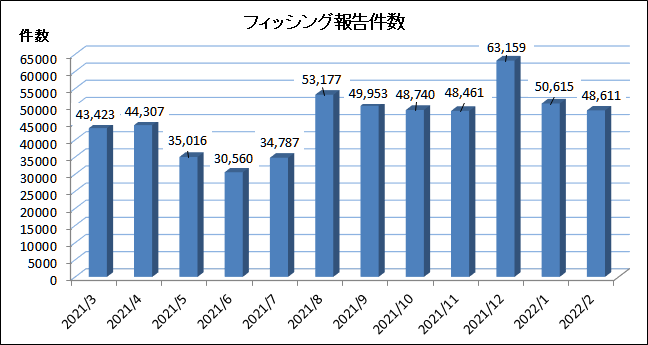
\includegraphics[width=12cm]{img/fishing.png}
                        \caption{2021年3月から2022年2月までのフィッシング報告件数 引用:フィッシング対策協議会}
                        \label{fishing}
                    \end{figure}
            \end{description}
            \clearpage
    \section{目標}
        本研究の目標を以下に示す.
        \begin{quote}
            偽のSSIDを用いた公衆無線LANからクライアントと正規サーバとの通信に割り込み,ブラウザに警告を出さずに通信の傍受・窃取を行う事.\
        \end{quote}
         ここで,ブラウザに警告を出さないという点について説明する.\
        Google Chromeによると,危険なコンテンツや詐欺的なコンテンツを検出すると,ブラウザ側で警告を表示するように設定されている.\
        Chromeの場合,以下の5つのどれかに該当した時に警告を出すように設定されている\cite{GoogleChromeHelp}.\
        \begin{enumerate}
            \item アクセスしようとしているサイトが,クライアントのデバイスに対して不正なソフトウェアをインストールさせようとしている場合.
            \item アクセスしようとしているサイトが,フィッシングサイトなどの偽のサイトである可能性がある場合.
            \item アクセスしようとしているサイトが,安全でない不審なサイトの可能性がある場合.
            \item アクセスしようとしているサイトが,Webブラウジングに問題を引き起こすようなプログラムをインストールさせようとしている場合.
            \item アクセスしようとしているサイトが,承認されていないソースからスクリプトを読み込もうとしている場合.
        \end{enumerate}
         検証の具体的な内容については以降の「前提条件と仮説」,「検証内容」で説明しているが,本研究ではクライアントと正規サーバとの通信の中継をする形で攻撃者を割り込ませている.\
        この時,正規サーバからの通信内容を複製してクライアントに提示する為,例えば上記の2や3などの項目に引っかかりクライアント側で警告を出される可能性がある.\
        警告が出ると,クライアント側にセキュリティ脅威を認知させる可能性が高くなる為,このような警告表示を出さない事を目標にした.\
    \section{前提条件と仮説}
        \subsection{前提条件}
            今回,MITM攻撃を仕掛けるにあたり以下の前提条件を設けた.\\
            \\
            利用者は
            \begin{itemize}
                \item 偽SSIDを有する無線LANアクセスポイント(以下,AP)を使用する.
                \item HTTPS通信で任意のサイトを閲覧する.
                \item 通信先を確認しない.
            \end{itemize}
             まず,偽SSIDを有するAPを利用するという前提条件について説明する.\
            攻撃者が利用者の通信の内容を盗み見る為には,利用者を攻撃者が用意したAPへ接続させる必要がある.\
            しかし,通常の公衆のAPのSSIDは,それを提供している施設や会社の名前に関連したものが多く,利用者も提供元の名前に関連したSSIDを有するAPに接続を試みる.\
            従って,攻撃者が用意したAPのSSIDも,利用者が施設や会社が提供したWiFiであると誤認させる様なSSIDを用いるという前提が必要である.\\
             次に,利用者はHTTPS通信でサイトを利用するという条件について,これは現在のWebサイト,特に個人情報やクレジットカード番号など機密性・重要性の極めて高い情報を扱うようなWebサイトは,常時HTTPS通信を用いている点にある.\
            特に,中間者攻撃への対抗策としてHSTP(HTTP Strict Transport Security)という,サーバーがブラウザに対してHTTPS通信を強制する様な仕組みが実装されているものもある.\
            従って,通信内容に対して暗号化が施されていないHTTP通信を前提としての検証は現実的でない為,HTTPS通信を想定する必要がある.\\
             最後に,通信先を確認しないという前提についてであるが,これは一般的な利用者の想定を意味する.\
            通常,ネットワークについての知識が深い利用者や,セキュリティリテラシーの高い利用者は,閲覧しているサイトのドメインの確認などを通して正規サーバとの通信を確認するが,一般的な利用者はそのような確認は行わない.\
            本研究は公衆無線LANを用いる一般的な利用者を想定している為,通信先の確認は想定しない.\\
        \subsection{仮説}
            上記の前提条件をもとに,次の仮説を立てた.
            \begin{quote}
                ユーザーが攻撃者が用意した偽のSSIDを有する公衆無線LANを用い,Captive Portalの仕様を用いて認証させた後,表示された偽の検索エンジンからネットを利用した場合,\
                ユーザーの通信がHTTPS通信でも,攻撃者がその通信の傍受・窃取が可能になる.
            \end{quote}
    \section{検証内容}
        \subsection{検証対象}
            MITM攻撃が可能か否かの検証にあたり,昨今急激な普及が見られるインターネット通販サイトを対象とした.その中でも国内ECモールの売上ランキング上位2つを占める「楽天」と「Amazon」を対象とした.\
            また,これ以降は,攻撃者が用意した悪意あるAPを「悪性AP」,通信の仲介に用いる攻撃者サーバを「悪性サーバ」をして説明する.
        \subsection{検証フロー}
            主な検証フローは次の通り.各フェーズの具体的な説明は次のサブセクションに記述している.
            \begin{enumerate}
                \item CaptivePortalを検知させて,予め攻撃者が用意しておいたCaptive Portalサイトに誘導し,認証を行わせる.
                \item 認証後,偽の検索エンジンの画面へ遷移させ,被害者が検索したワードを悪性サーバで取得する.
                \item 攻撃者は取得したワードをバックエンドで検索し,その検索結果を取得する.
                \item 取得したHTMLファイル内にあるハイパーリンクを書き換え,そのコピーを被害者に提示する.
                \item 以後,クリックしたURLを悪性サーバで取得する.
                \item 攻撃者は取得したURLを利用して正規サーバにアクセスする.
                \item 正規サーバから返却されたHTMLファイル内のハイパーリンクを書き換えたものを被害者に提示する.
            \end{enumerate}
        \subsection{実装}
            悪性サーバの実装はGolangで実装した.\
            付録に該当のGitHubリポジトリのリンクを載せている.\
            ここでは,各検証フローについて具体的な実装内容を示す.\
            \subsubsection{検証フロー1,2について}
                前提知識・用語のセクションでも記述したが,Captive Portalとは,インターネットを利用する際にそのユーザーの認証や利用規約に同意させる為に,一時的に外部との通信を制限して認証画面に飛ばす仕組み,或いはその認証ページを指す.\
                例えばカフェや飛行機,新幹線で提供されている公衆無線LANを利用した際などは,認証ページに飛ばされるという経験は決して珍しいものではない.\
                また,要求された認証が終えると,インターネットへのアクセスが許可され,予め用意された別のサイトに飛ばされる事もある.\
                今回はこの仕組みを利用する(図\ref{flow-no12}).\
                \begin{figure}[pth]
                    \centering
                    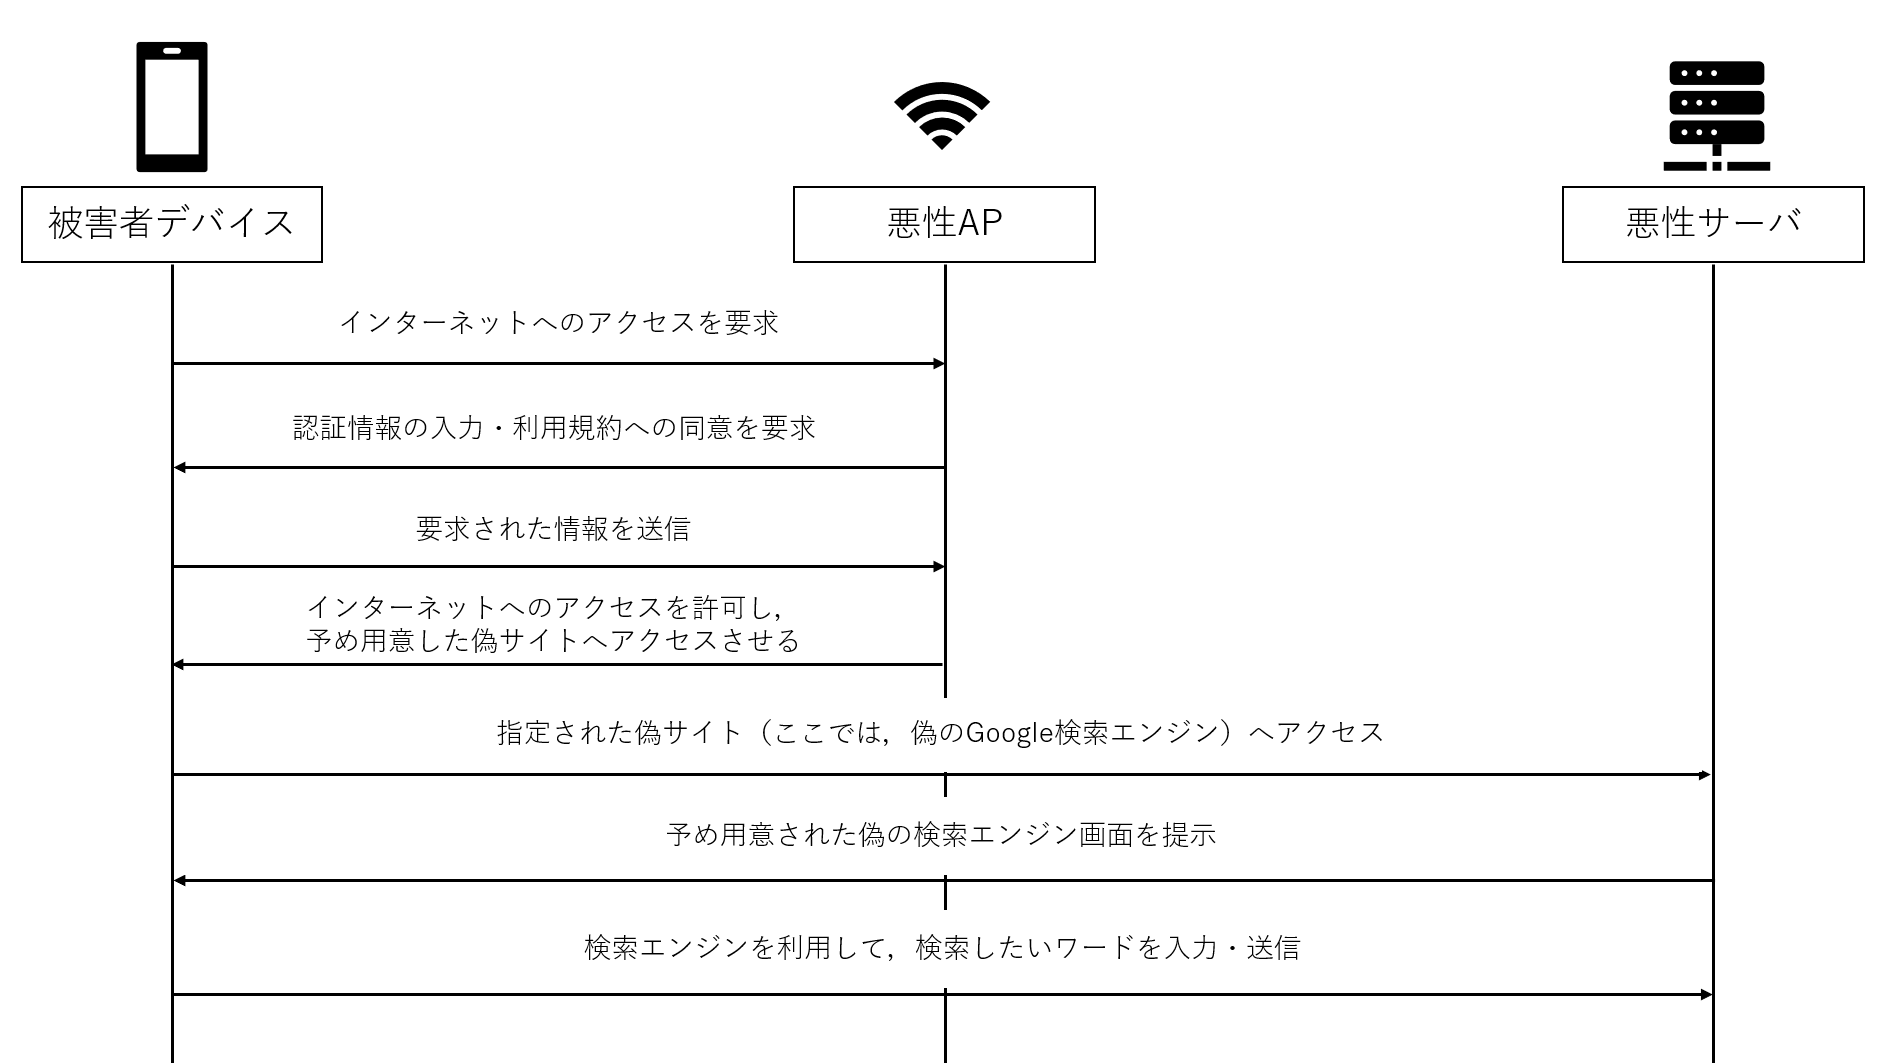
\includegraphics[width=12cm]{img/vc-vf-1-2.png}
                    \caption{偽のAPとCaptive Portalの仕組みを仕様して,偽の検索エンジンに飛ばすまでの挙動}
                    \label{flow-no12}
                \end{figure}
                \clearpage
            \subsubsection{検証フロー3について}
                ここでは,最も利用されているGoogleの検索エンジンを用いた.\
                Googleでの検索結果を取得する為には,検索クエリを作成する必要がある.\
                基本的に任意のクエリ(query)に対して https://google.com/search?q=queryというURLがGoogleの検索URLとなっているが,クエリに空文字列が存在する場合は,その空文字列を+に置換する必要があることに留意しなければならない.\
                例えば,「神戸大学 工学部」と検索する場合には,そのURLはhttps://google.com/search?q=神戸大学+工学部となる.\
                このURLを叩くことで,正規サーバからの応答を取得・自動生成を行う(図\ref{flow-no3}).\\
                \begin{figure}[pth]
                    \centering
                    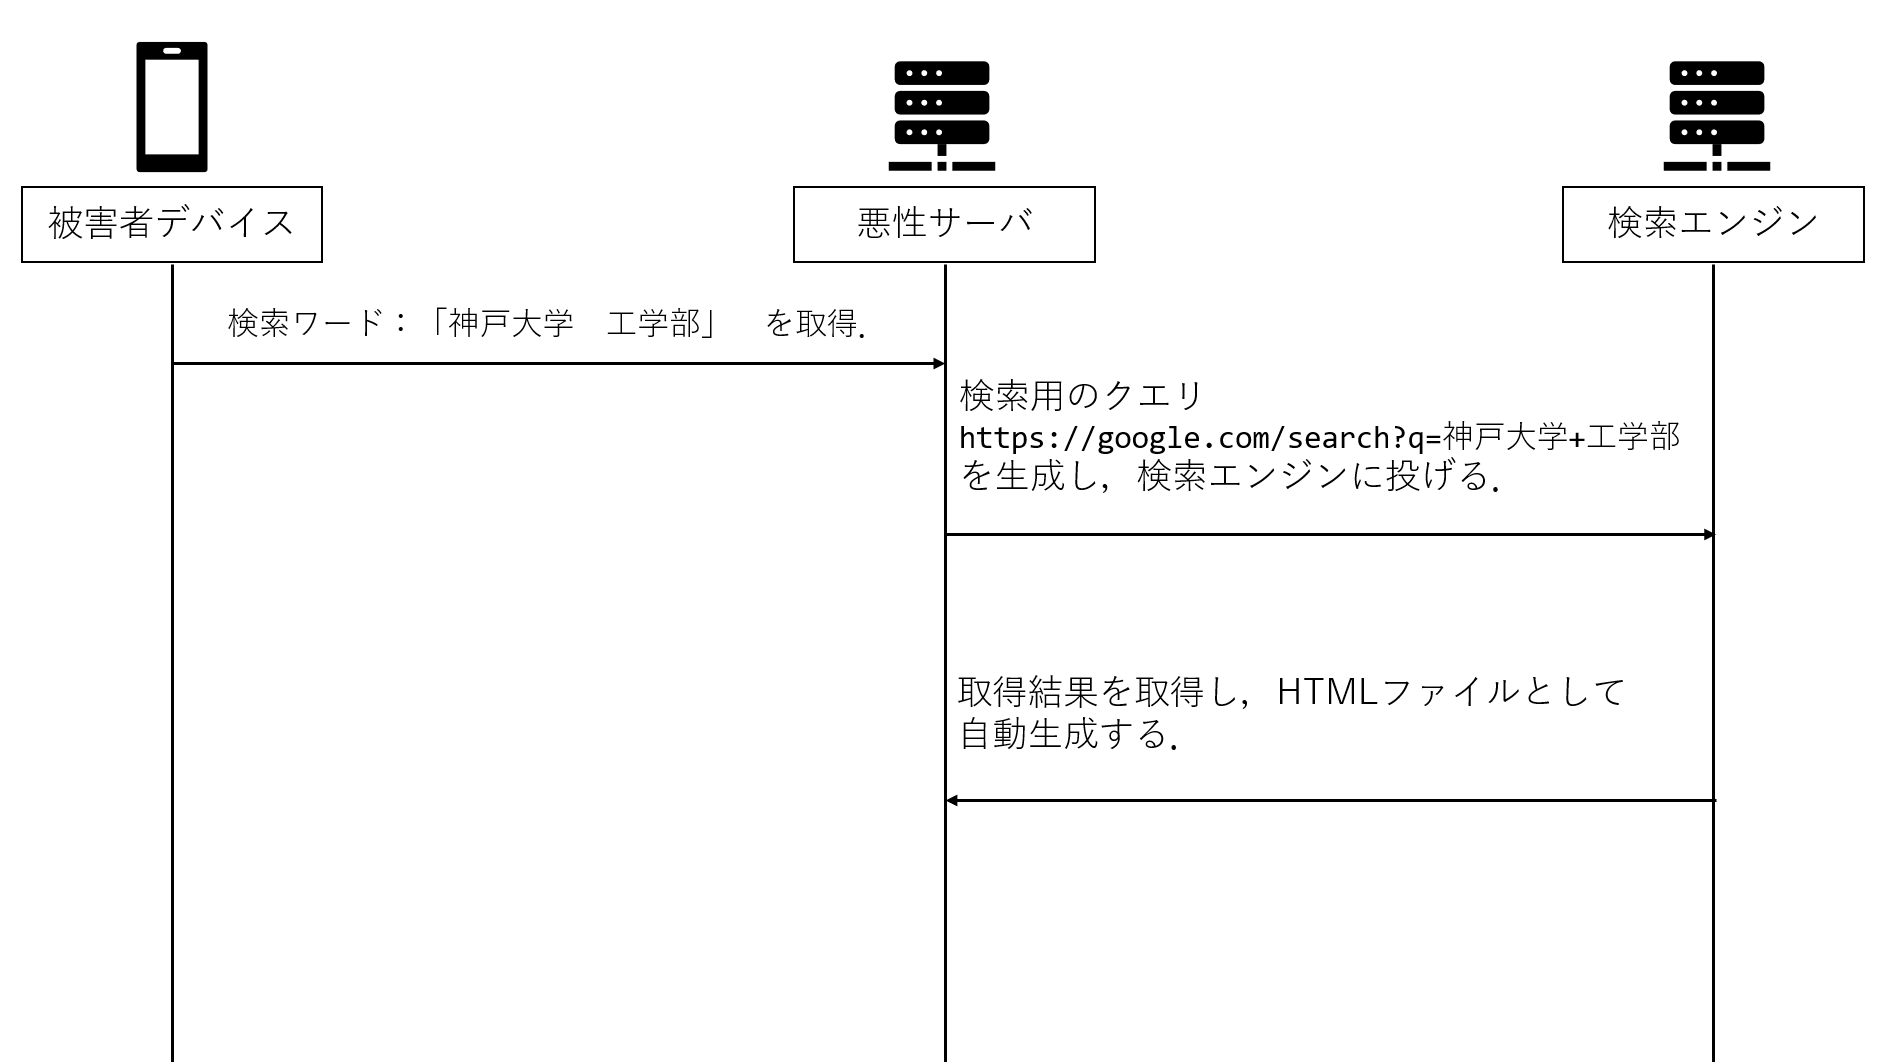
\includegraphics[width=12cm]{img/vc-vf-3.png}
                    \caption{検索ワードを取得してから,検索結果を取得するまでの流れ}
                    \label{flow-no3} 
                \end{figure}
                \clearpage
            \subsubsection{検証フロー4,5について}
                取得したHTMLファイル内にあるハイパーリンクがそのままであれば,悪性サーバではなく正規サーバとの通信に切り替わってしまう(図\ref{flow-no45-00}).\
                従って,既存のURLを悪性サーバへ通信するように書き換え,且つ既存のURLを正確に抽出する必要がある.\
                これを実現する為には,既存のハイパーリンクをルールに則って書き換える必要がある.\
                具体的に,https://example.comというURLに対して処理を行うことを考える.\
                サーバには予め,URLを受け取る為のエンドポイントを設置する.今回の場合は「/templates」というエンドポイントに対して,「url」というパラメータを受け取るものとする.\
                このエンドポイントに対して適切にURLを飛ばすために,サーバ側で予め/templates?url=https://example.comのように書き換える.\
                その結果,被害者に提示したHTMLファイル内にあるハイパーリンクをクリックすると悪性サーバに飛び,且つサーバ側で遷移しようとしたページのリンクを取得できる(図\ref{flow-no45-01}).
                \begin{figure}[pth]
                    \centering
                    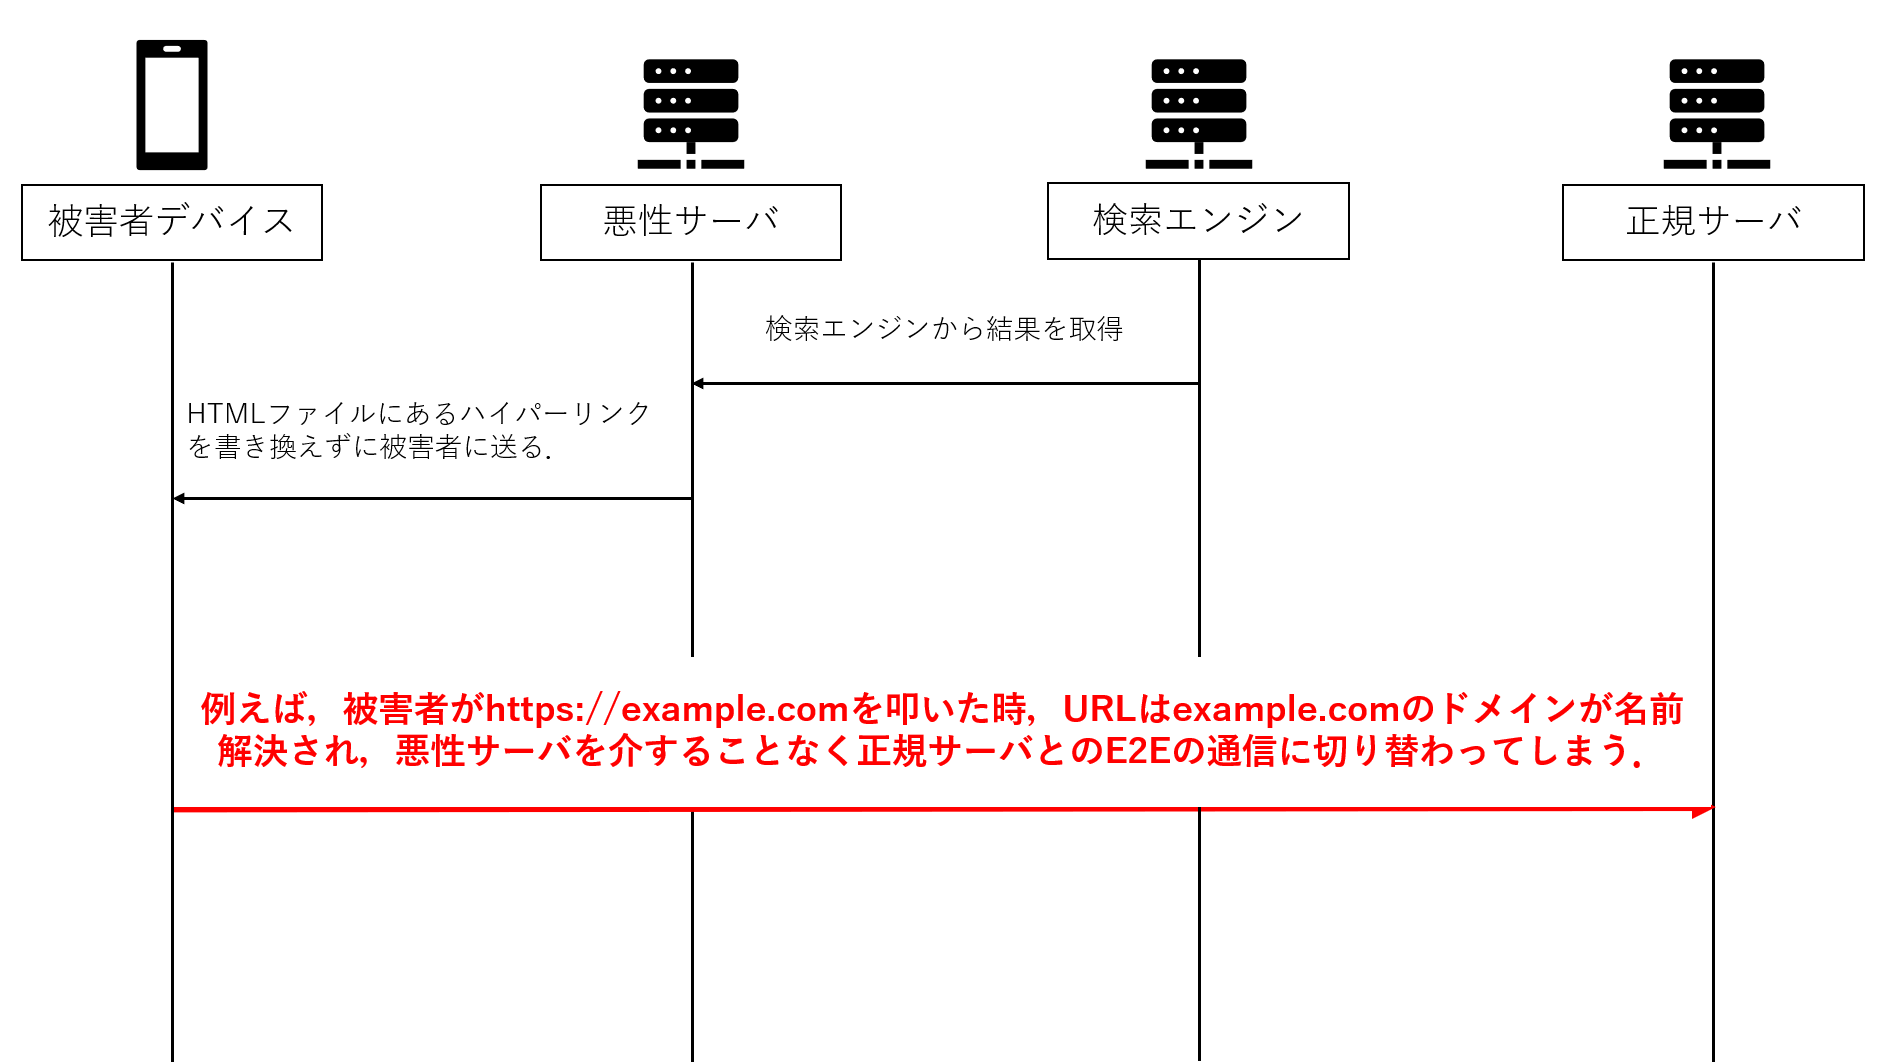
\includegraphics[width=12cm]{img/vc-vf-4-5-00.png}
                    \caption{HTMLファイル内のハイパーリンクを書き換えなかった場合の挙動}
                    \label{flow-no45-00}
                    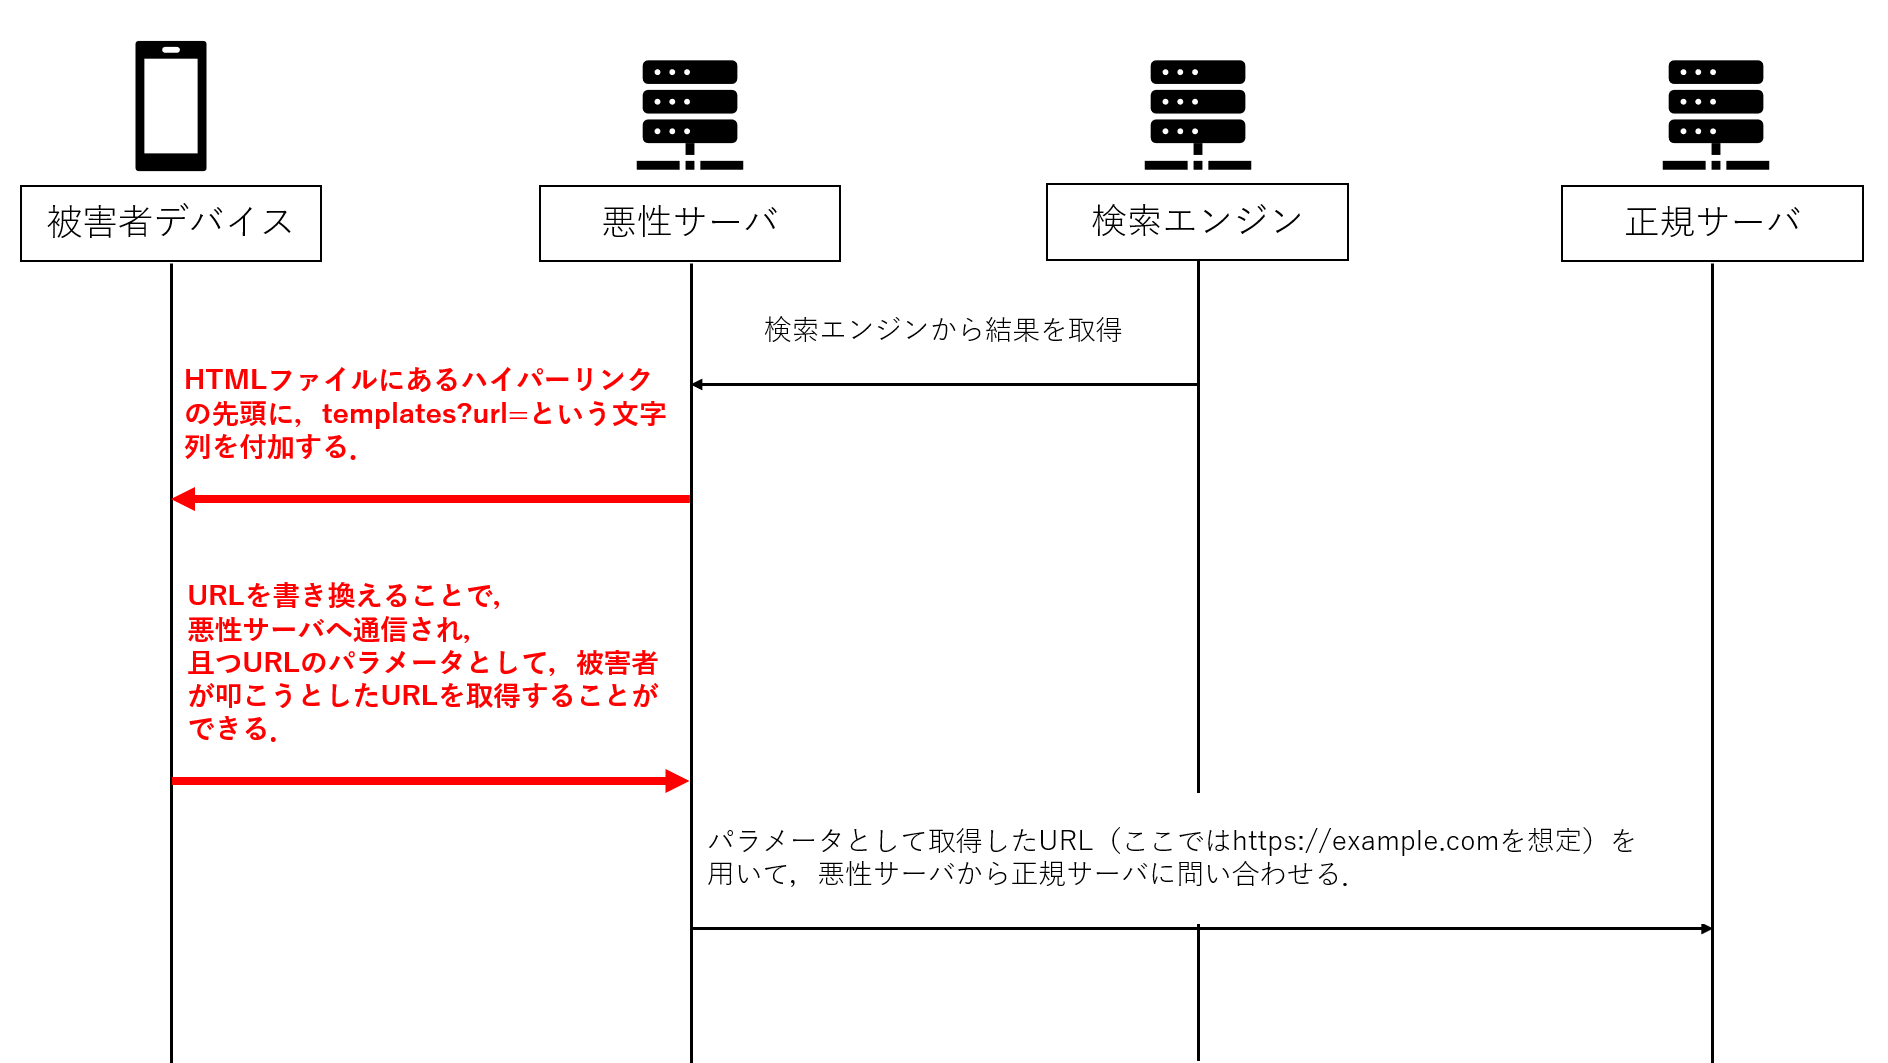
\includegraphics[width=12cm]{img/vc-vf-4-5-01.png}
                    \caption{HTMLファイル内のハイパーリンクを書き換えた場合の挙動}
                    \label{flow-no45-01}
                \end{figure}
                \clearpage
            \subsubsection{検証フロー6,7について}
                フローの4と5で得た正規URLを用いて,バックエンドで正規サーバとの通信及びHTMLファイルの取得を行う.\
                通常の通信であればHTMLファイルの取得のみでよいが,個人アカウントへのログインを行う際は,そのIDとパスワードを取得し且つ得られた情報と実際に登録されている情報との整合性の確認を行わなければならない.\
                登録情報の整合性に関しては,取得した個人情報を攻撃者が手動で入力・確認を行わず,バックエンドでブラウザのインスタンスを生成して入力・確認を行う.\
                この処理に関して,ChromedpというGolangで実装されているパッケージを用いた(付録10.2参照) .\
                具体的な実装については付録からGitHubレポジトリを参照して頂きたい.ここでは,処理の流れを以下に簡単に示す.\
                \begin{enumerate}
                    \item Chromeインスタンスを生成する.
                    \item 指定URLを叩き,JS Pathを指定して該当部分に取得したIDやパスワードを入力する.
                    \item 個人情報の入力が完了すれば,同じくログインボタンのJS Pathを指定してログイン処理を行う.
                    \item 正規サーバに情報を整合させ,返却されたHTMLファイル内のハイパーリンクを,4と5と同じ要領で書き換えて被害者に返却する.
                \end{enumerate}
                JS Pathの指定に関しては,予め正規サイトのログイン画面を見てから確認・指定をする必要がある.\
                \begin{figure}[pth]
                    \centering
                    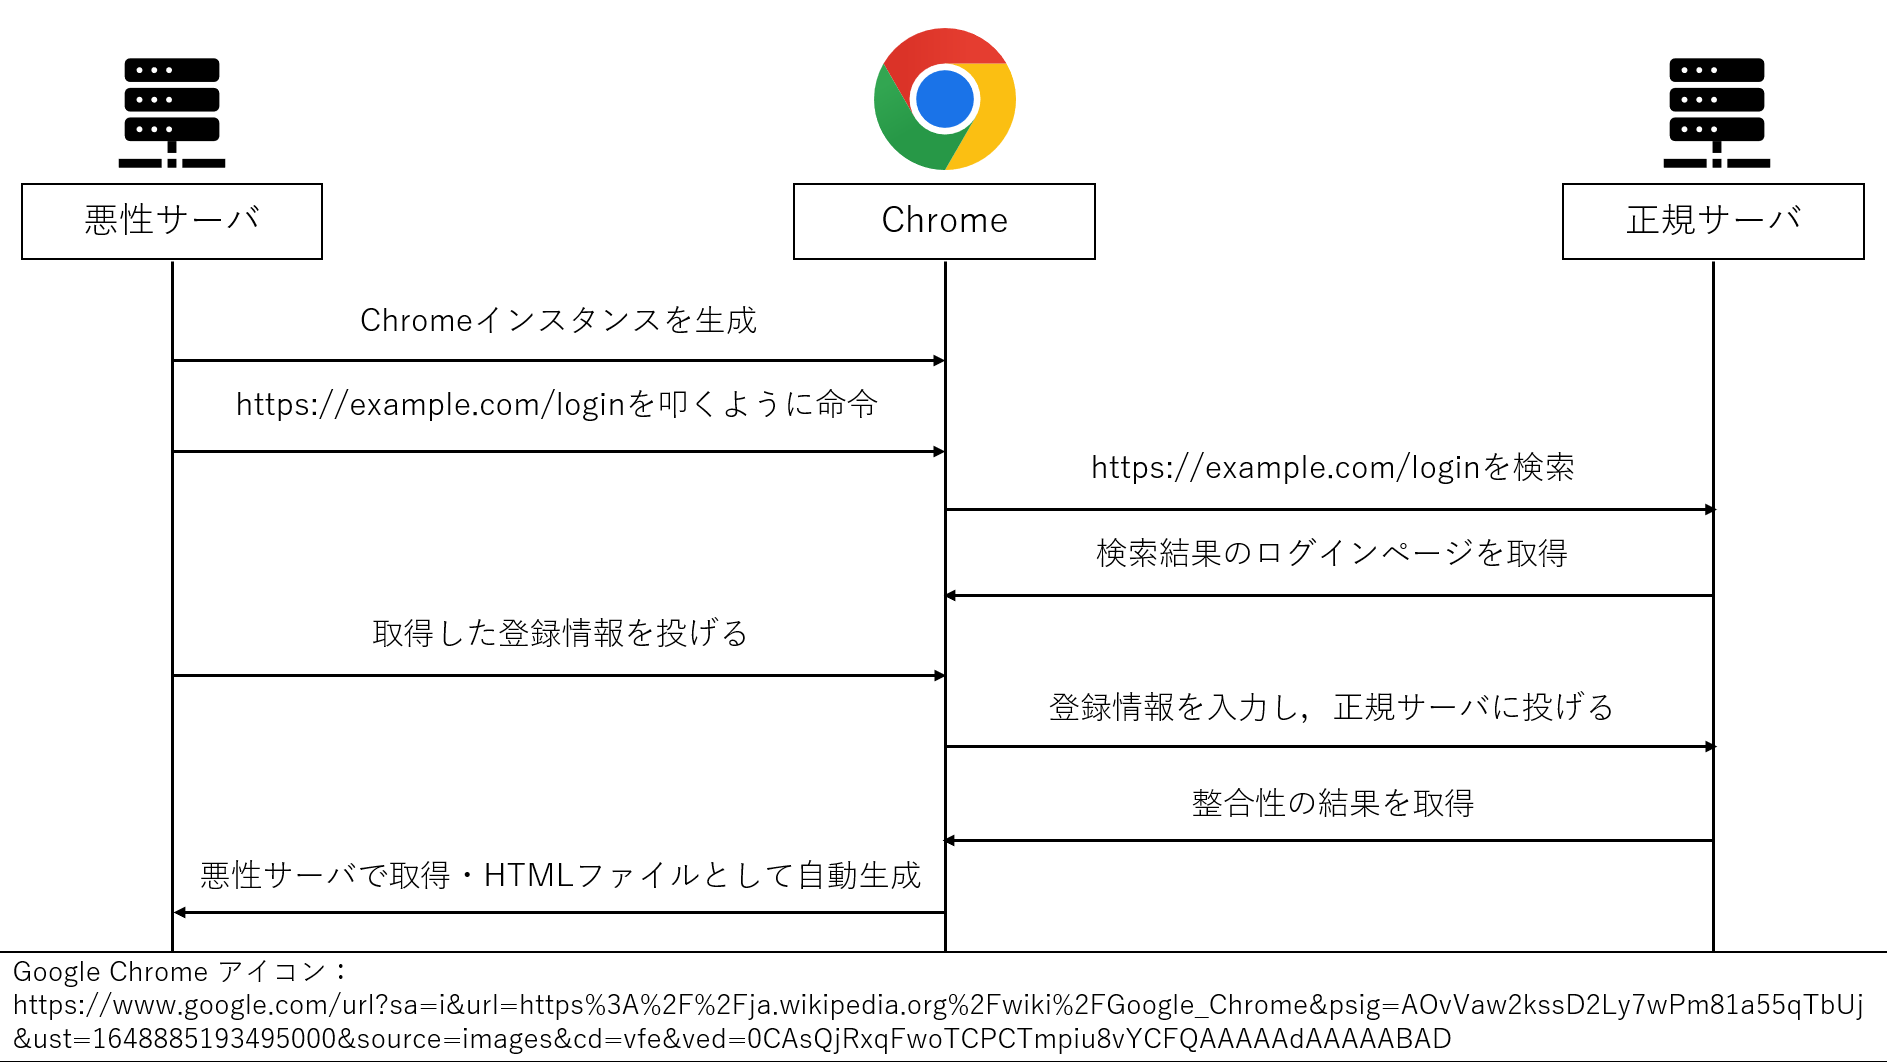
\includegraphics[width=12cm]{img/vc-vf-6-7.png}
                    \caption{登録情報の整合性の確認を行う流れ}
                    \label{flow-6-7}
                \end{figure}
                \clearpage
        \section{検証結果}
            検証結果は以下のようになった.
            \subsection{楽天の場合}
                \subsubsection{動作結果}
                    まず,認証画面への遷移し(図\ref{rakuten-00}),認証が終了すると偽の検索エンジンが表示される(\ref{rakuten-01}).\
                    ここの検索欄に「楽天通販」と検索して,その検索結果を待つ.\
                    \begin{figure}[pth]
                        \centering
                        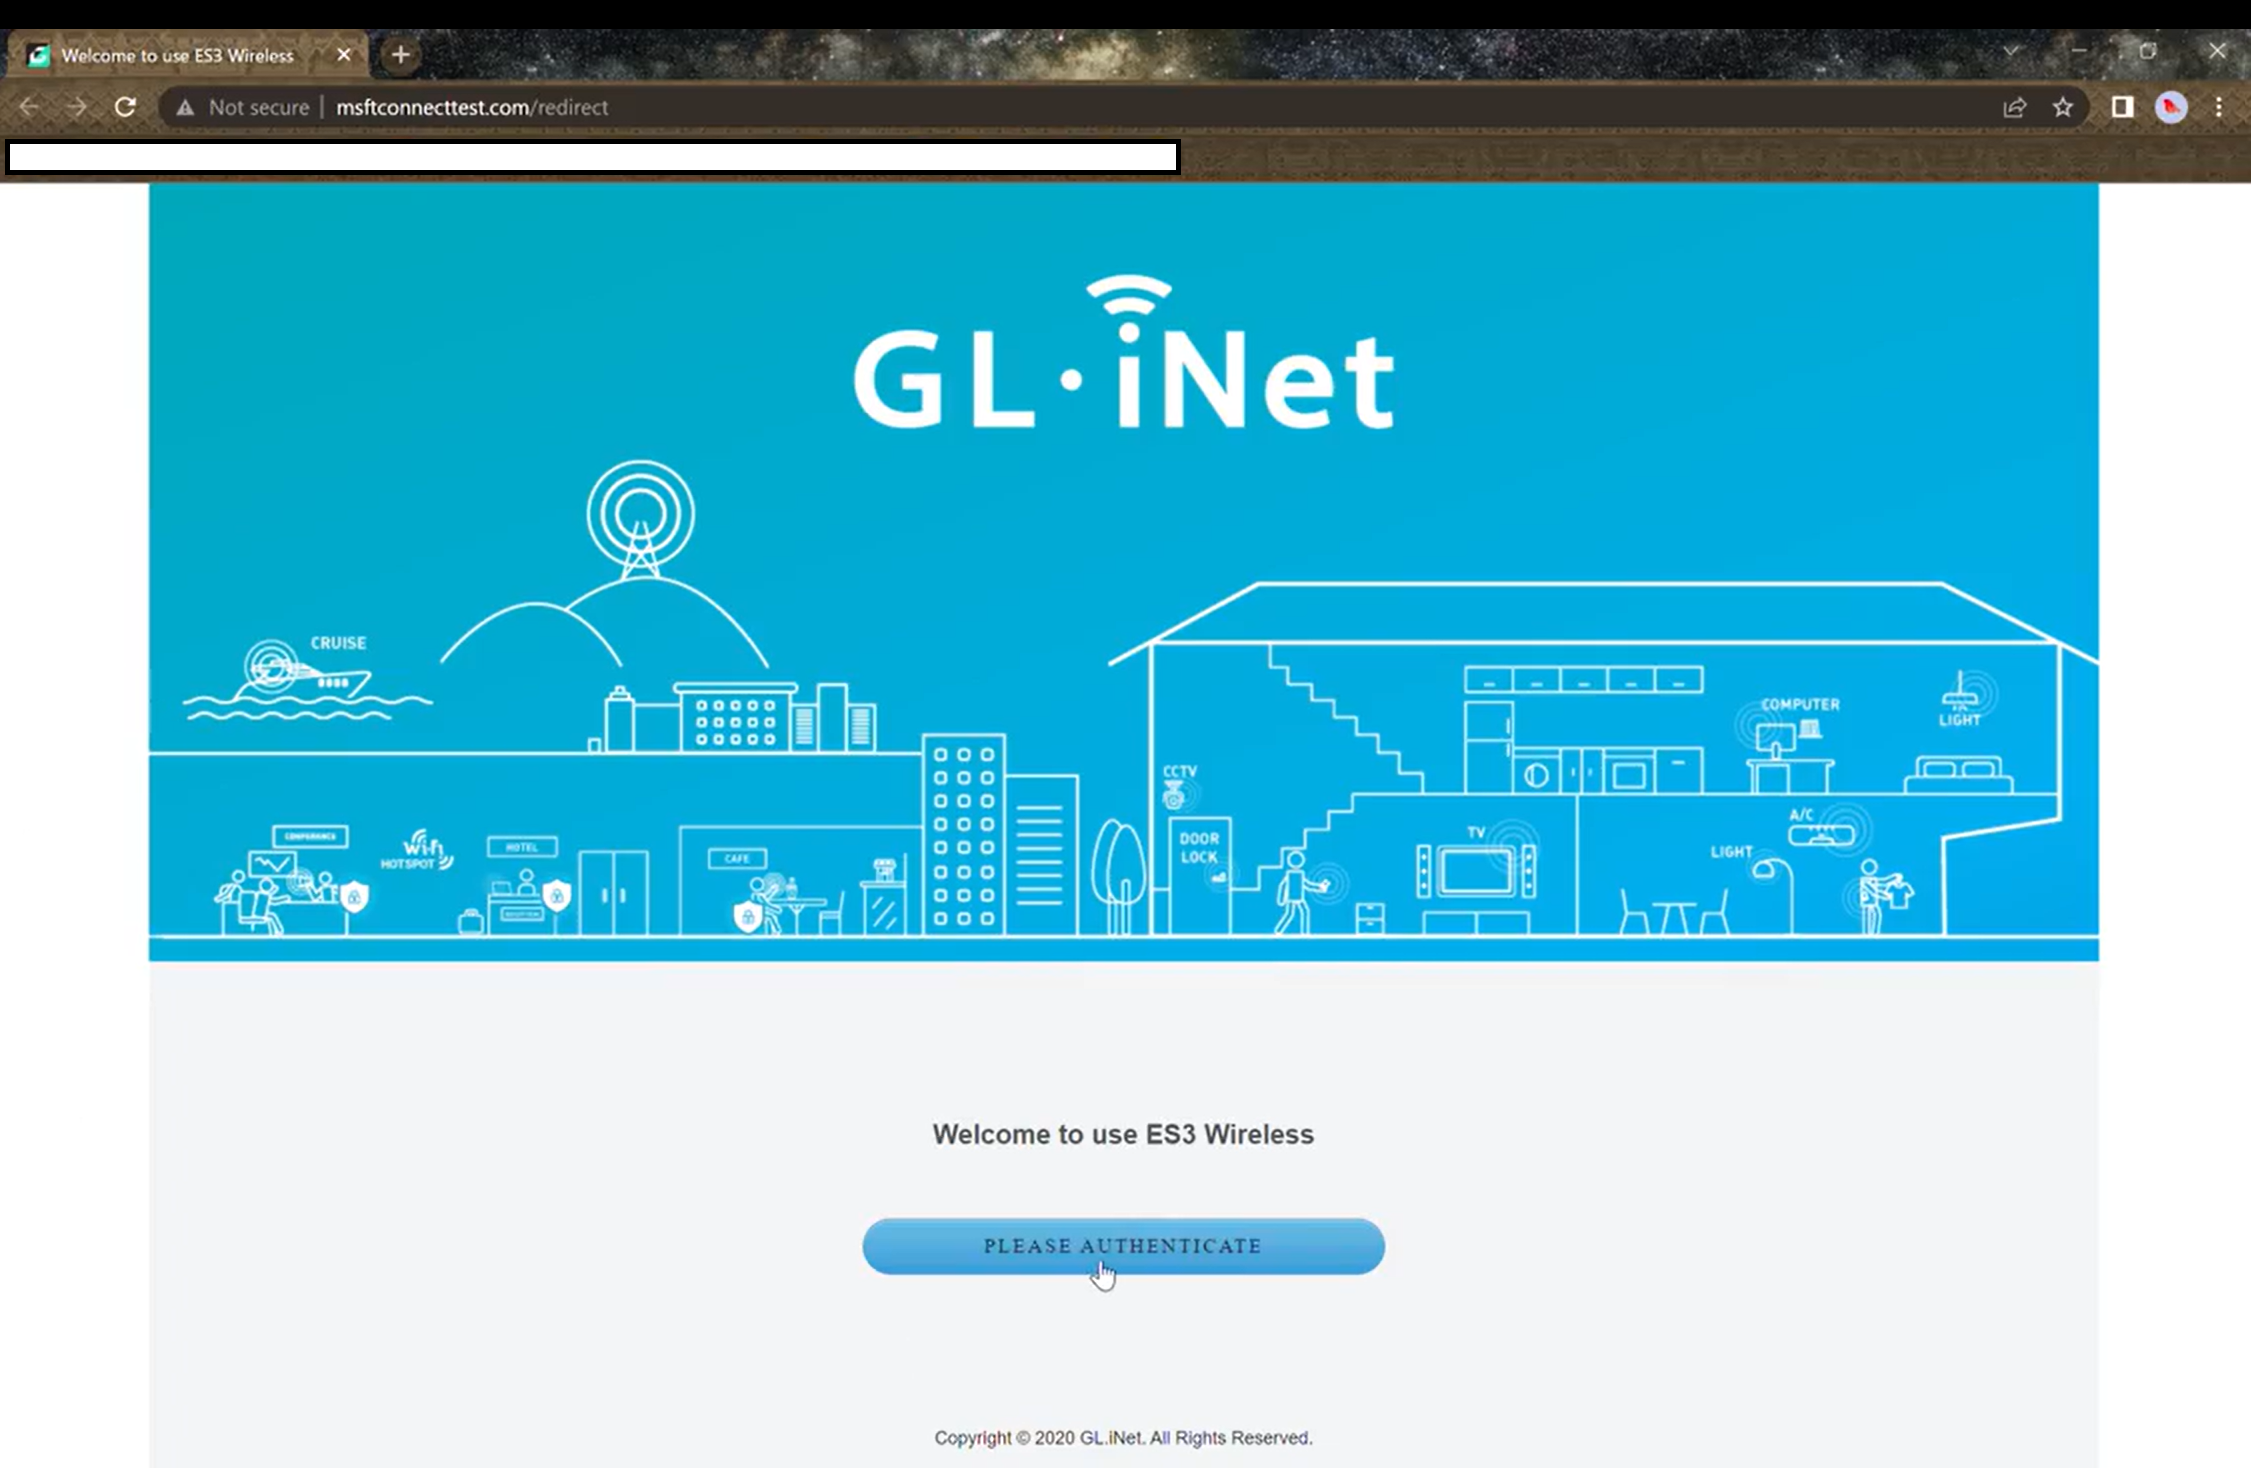
\includegraphics[height=7cm]{img/rakuten/rakuten-00.png}
                        \caption{認証画面}
                        \label{rakuten-00}
                    \end{figure}
                    \begin{figure}[pth]
                        \centering
                        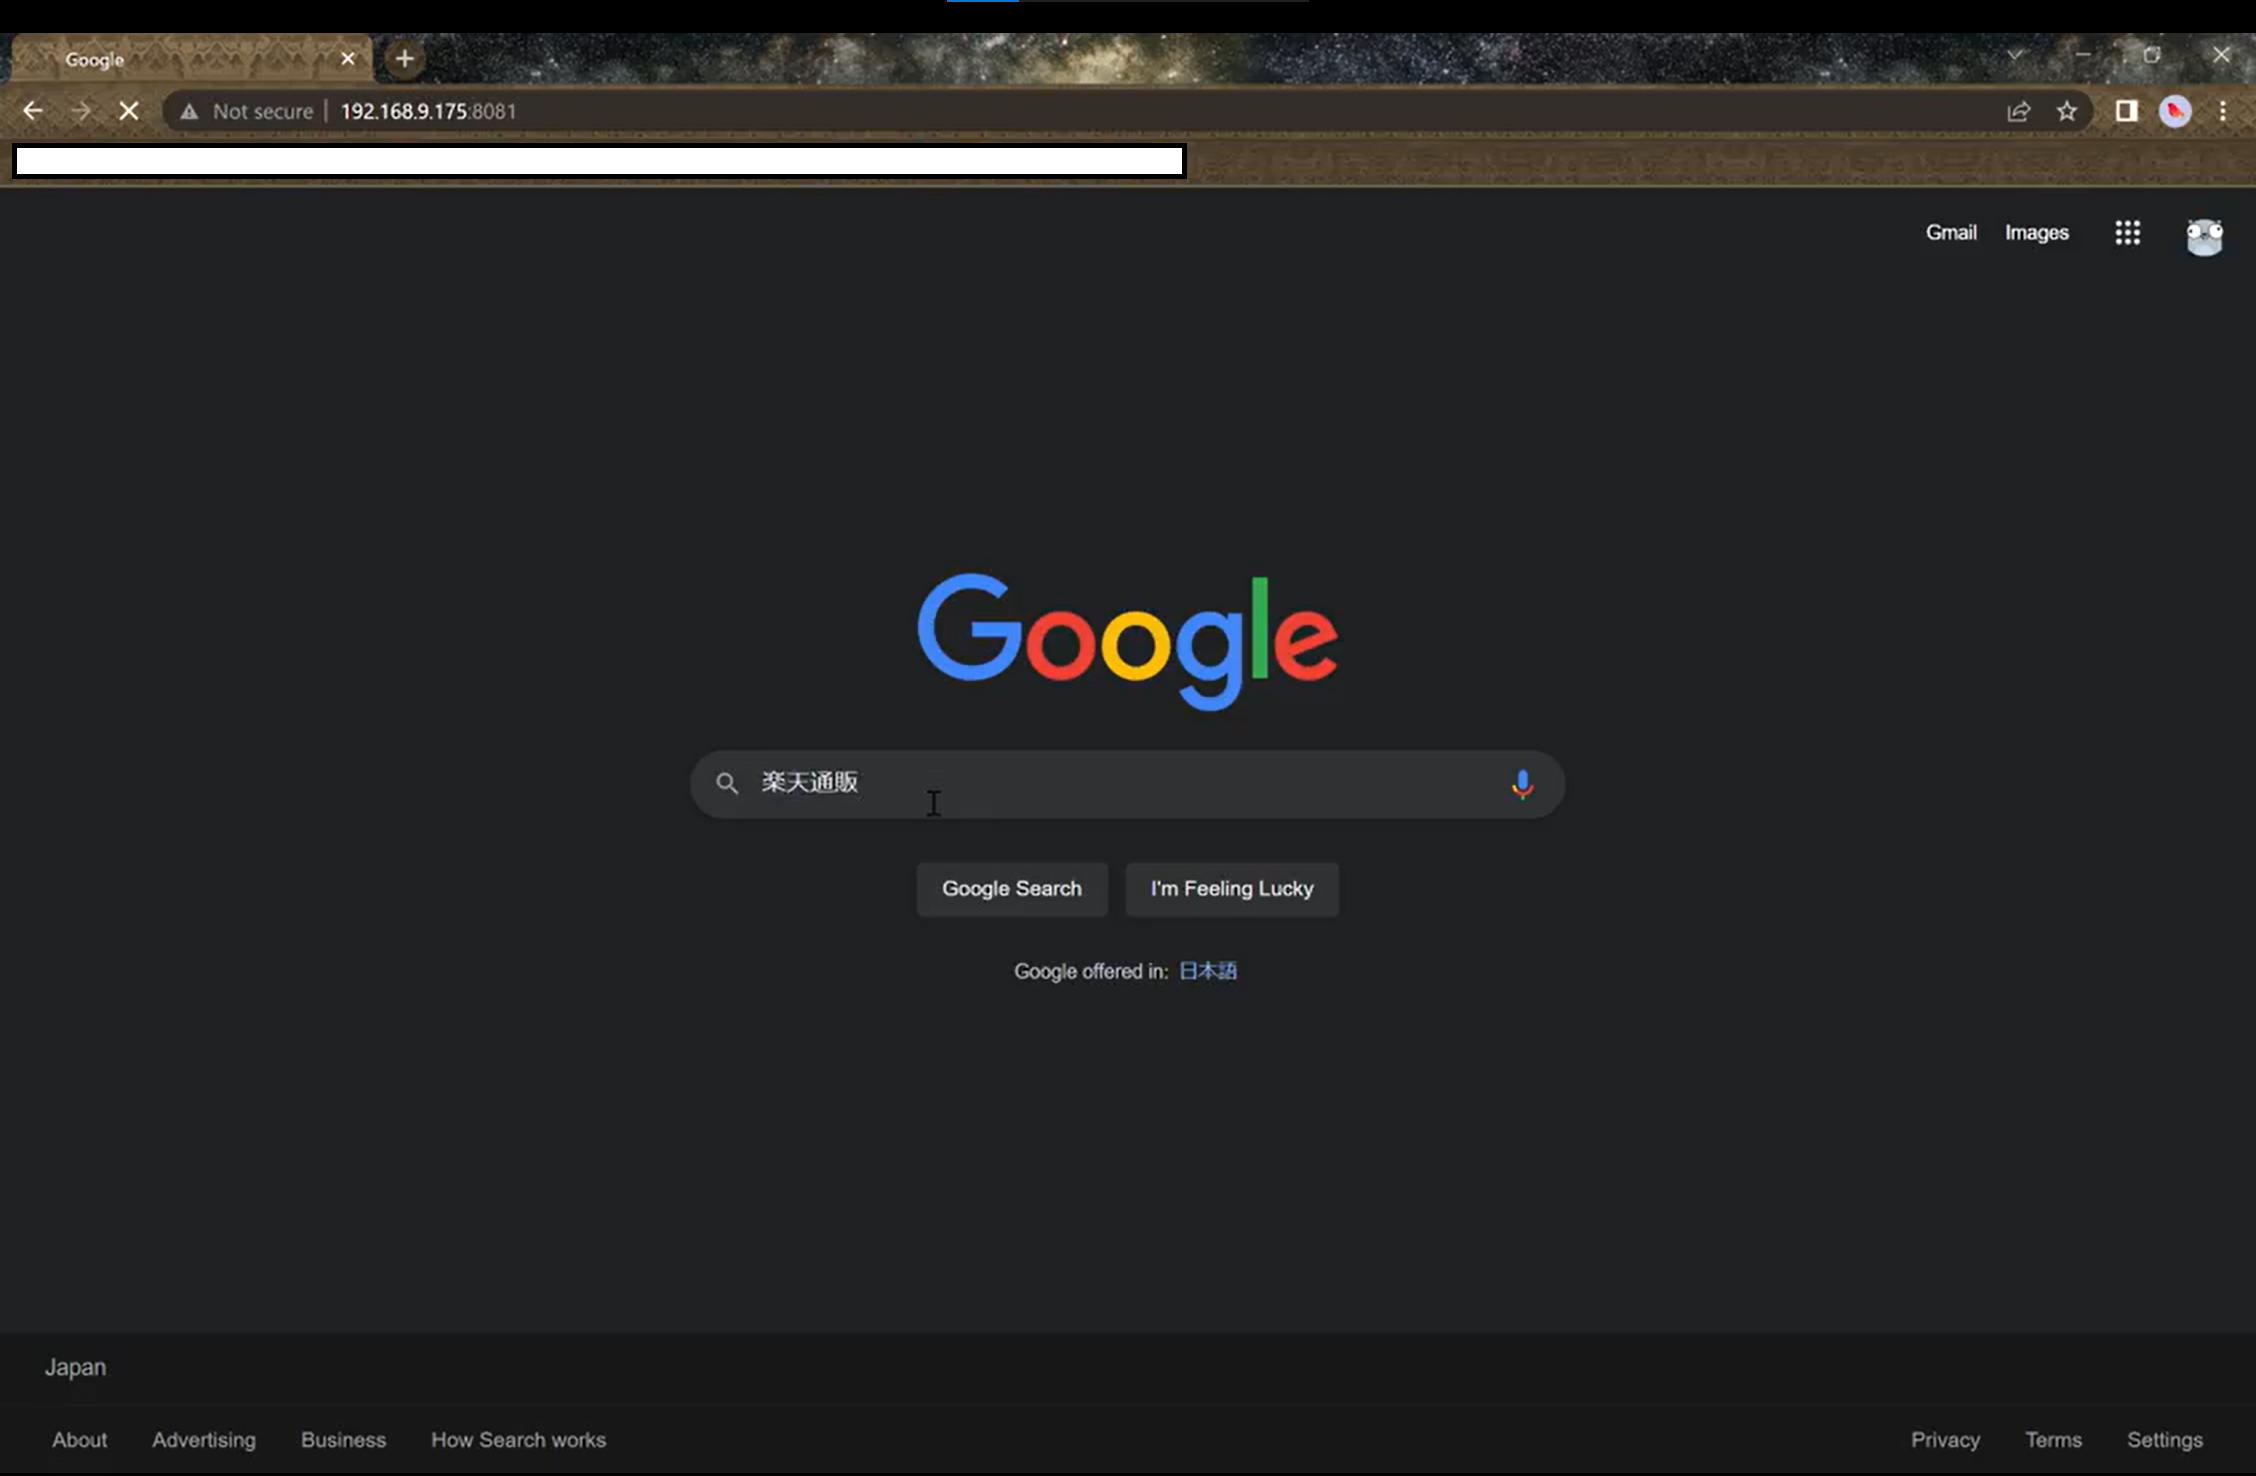
\includegraphics[height=7cm]{img/rakuten/rakuten-01.png}
                        \caption{偽のGoogle検索画面}
                        \label{rakuten-01}
                    \end{figure}
                    \clearpage
                    「楽天通販」と検索して得られた結果を表示する(図\ref{rakuten-02}).\
                    ここで,被害者はGoogleの検索結果が得られたものと認識し,表示された楽天通販の結果から該当のサイトへのリンクをクリックする.\
                    ここまでの動作は,図\ref{flow-no45-01}に準じて処理されたものである.\
                    \begin{figure}[pth]
                        \centering
                        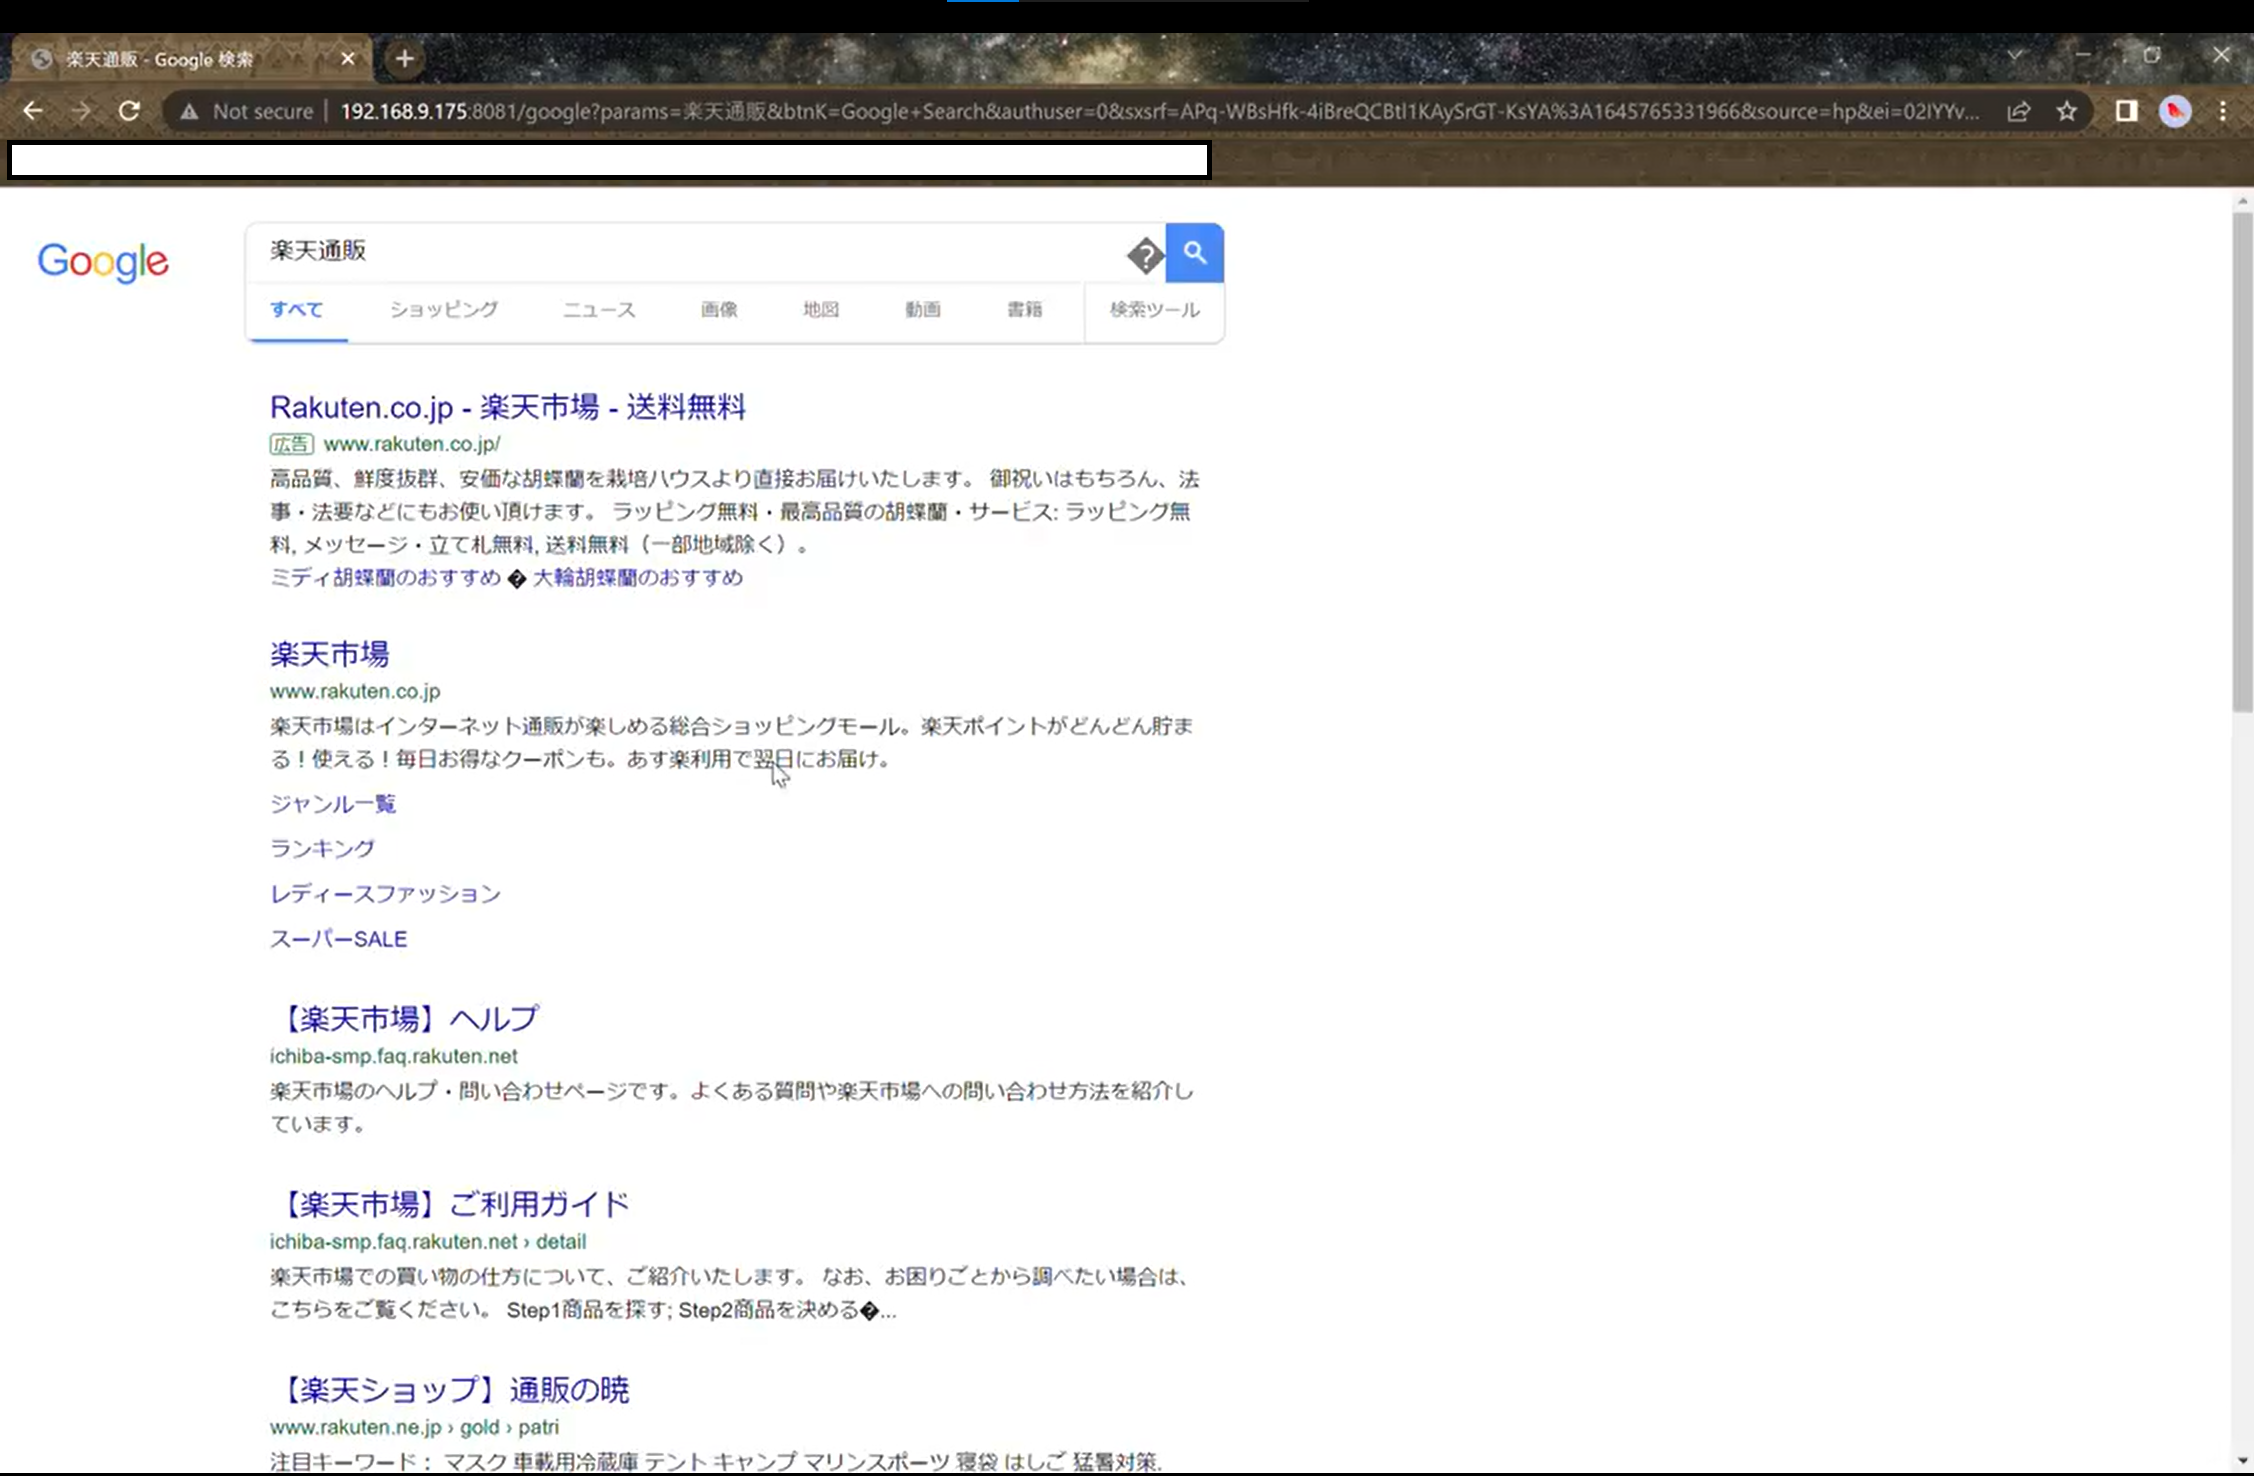
\includegraphics[height=7cm]{img/rakuten/rakuten-02.png}
                        \caption{「楽天通販」と検索した際の画面}
                        \label{rakuten-02}
                    \end{figure}
                    \\
                     得られて検索結果の画面から,楽天通販サイトに入る.\
                    特に目立った文字化けや画像切れは起こっていない事から,ここまでも被害者は.楽天通販サイトに遷移したと認識する物とする.\
                    ここで,個人アカウントに入る為に「ログイン」ボタンを押す(図\ref{rakuten-03}).\
                    \begin{figure}[pth]
                        \centering
                        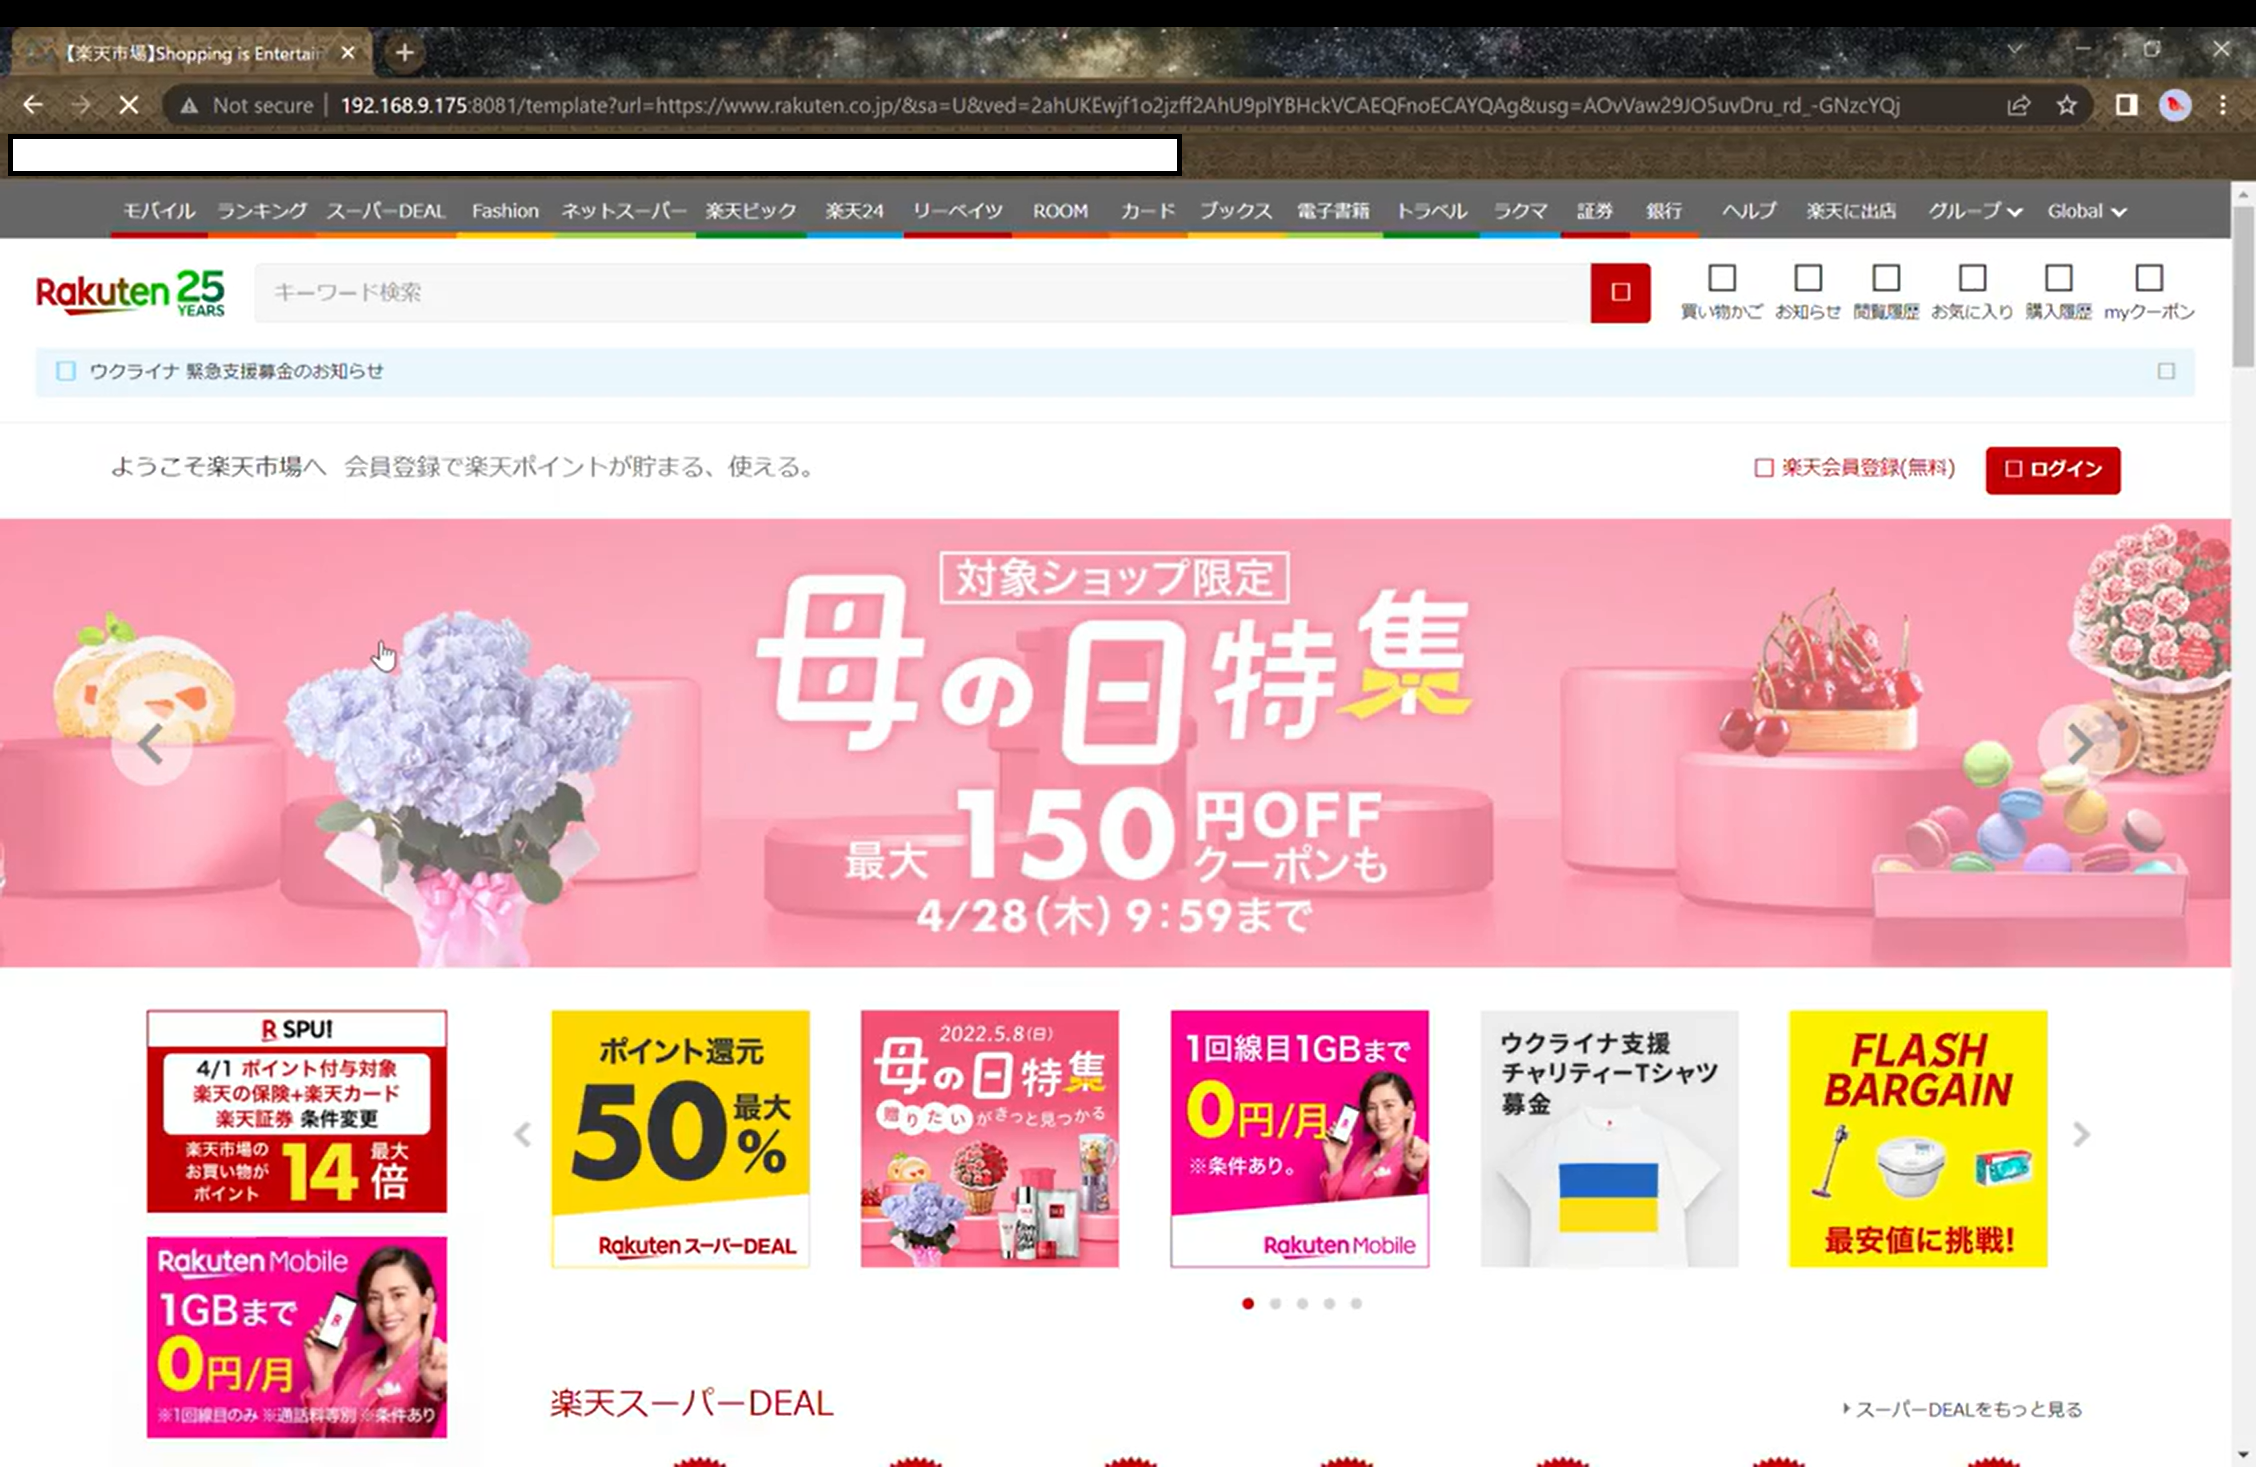
\includegraphics[height=7cm]{img/rakuten/rakuten-03.png}
                        \caption{検索結果の画面から楽天の複製サイトへ侵入した際の画面}
                        \label{rakuten-03}
                    \end{figure}
                    \clearpage
                    「ログイン」ボタンを押した結果は以下のようになる(図\ref{rakuten-04}).\
                    このログイン画面は,攻撃が予め用意して攻撃者サーバにパラメータを送信させるように実装されたものである.\
                    ここに,実際に自分のアカウント情報を入力し,「ログイン」ボタンを押す.\
                    \begin{figure}[pth]
                        \centering
                        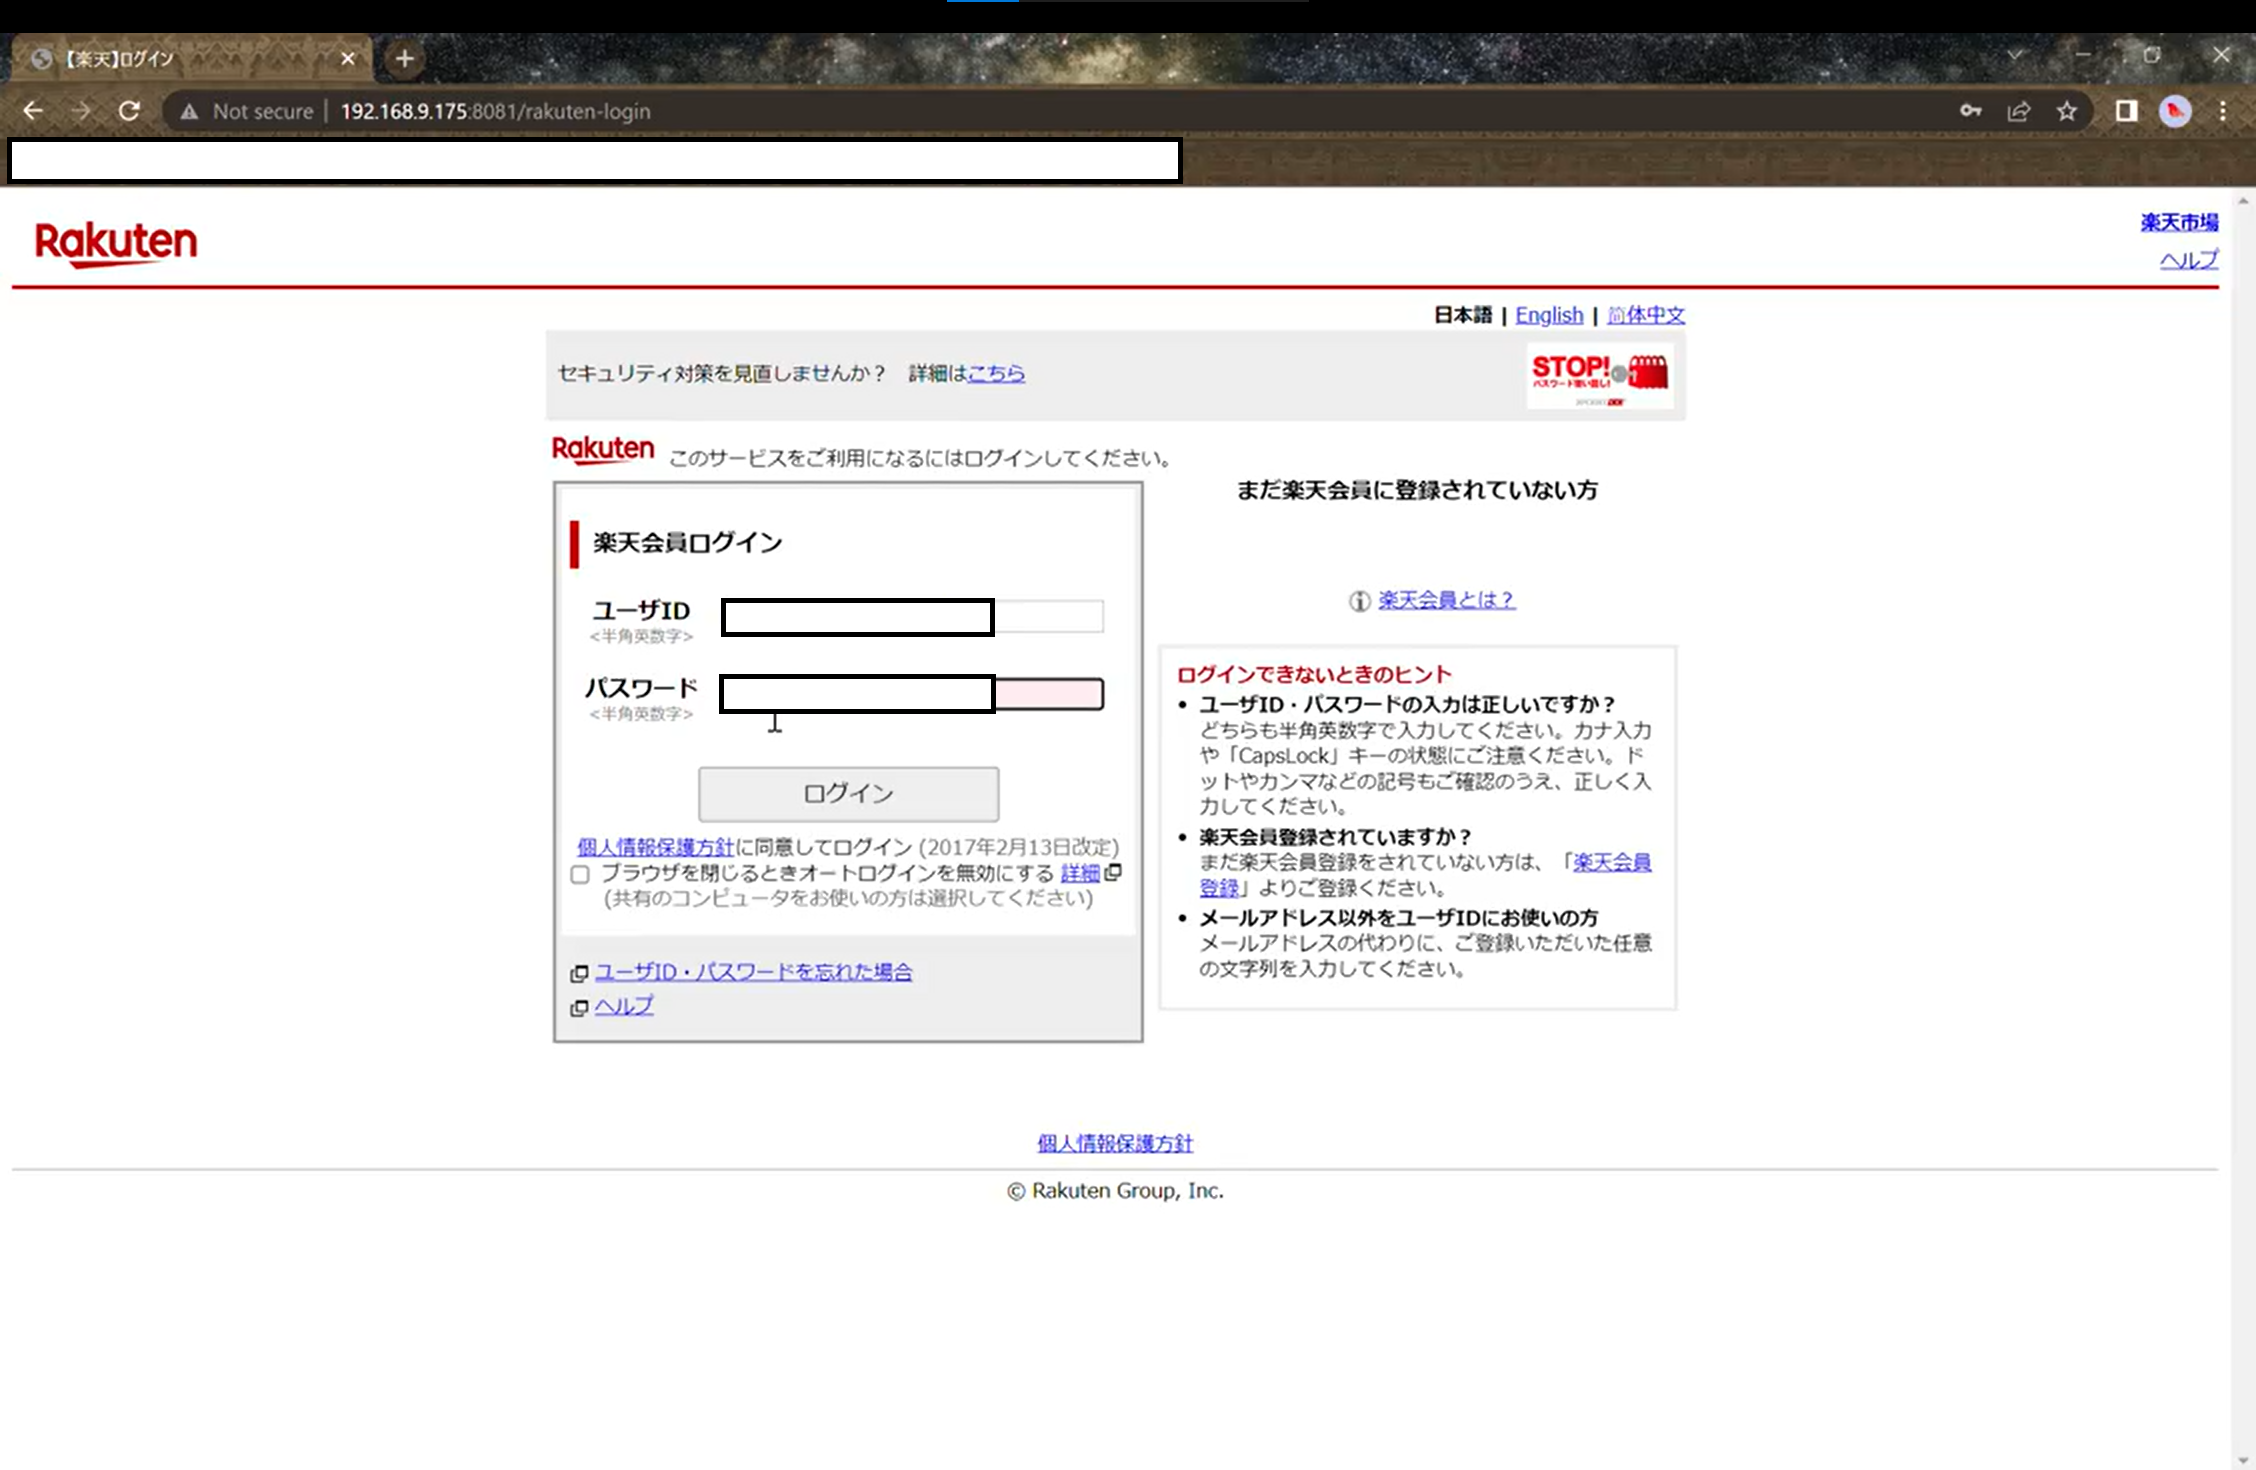
\includegraphics[height=7cm]{img/rakuten/rakuten-04.png}
                        \caption{ログイン画面へ入り,登録情報を入力した際の画面}
                        \label{rakuten-04}
                    \end{figure}
                    \\
                     入力されたパラメータを攻撃者サーバ内から処理をし,正規サーバから返却された結果を被害者に提示する.\
                    図\ref{rakuten-05}は,実際に個人アカウントに侵入した結果である.\
                    ここまでの動作は図\ref{flow-6-7}に準じて処理されており,目立った警告や画像切れ無く且つ正規サーバとの通信を中継する形で個人アカウントへのログインに成功した.\
                    \begin{figure}[pth]
                        \centering
                        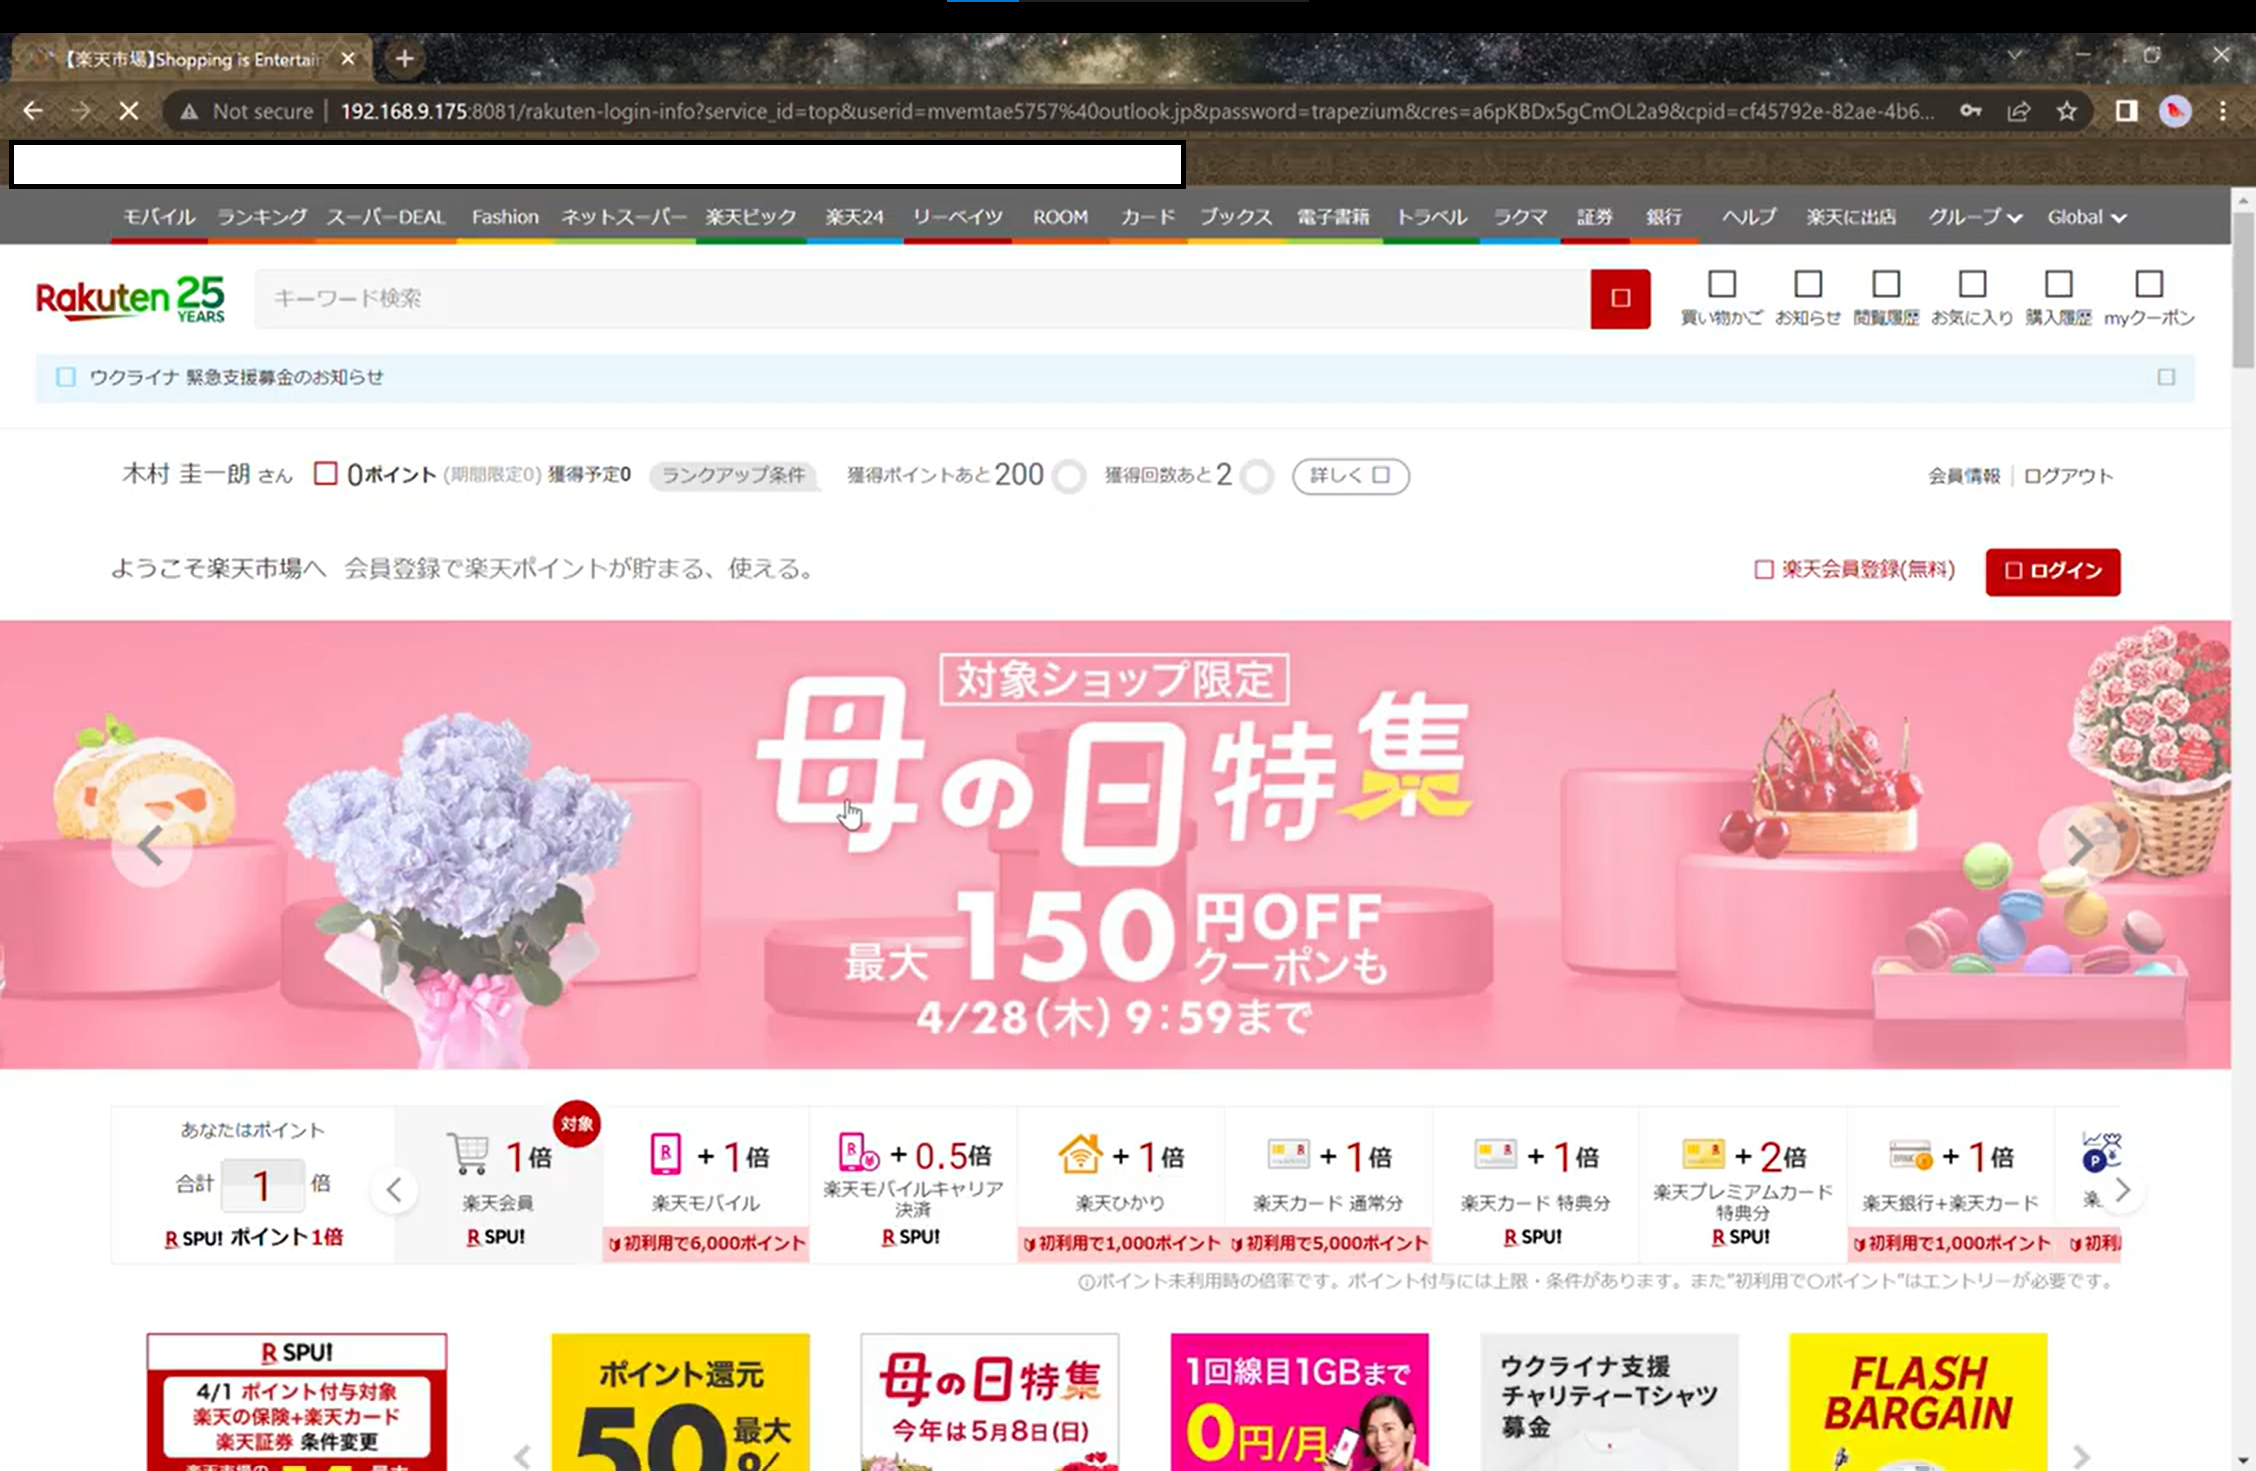
\includegraphics[width=7cm]{img/rakuten/rakuten-05.png}
                        \caption{ログイン情報の整合が取れ,実際に個人アカウントへログインした後の画面}
                        \label{rakuten-05}
                    \end{figure}
                    \clearpage
                \subsubsection{問題点}
                    楽天の場合の主な問題点として,ログイン情報の入力から実際にログインが完了されるまで,ある程度の時間を要する事が挙げられる.\
                    具体的な実行時間の結果を\ref{calc-run-time}に示す.\
                    \begin{table}[pth]
                        \centering
                        \caption{Amazonと楽天の実行時間比較}
                        \begin{tabular}{lll}
                        \hline
                             & 楽天           & Amazon      \\ \hline
                        1回目  & 24.73{[}s{]} & 6.64{[}s{]} \\
                        2回目  & 24.65{[}s{]} & 6.98{[}s{]} \\
                        3回目  & 24.43{[}s{]} & 7.30{[}s{]} \\
                        4回目  & 24.81{[}s{]} & 7.35{[}s{]} \\
                        5回目  & 24.43{[}s{]} & 7.27{[}s{]} \\
                        6回目  & 24.86{[}s{]} & 7.55{[}s{]} \\
                        7回目  & 24.37{[}s{]} & 7.51{[}s{]} \\
                        8回目  & 25.43{[}s{]} & 7.45{[}s{]} \\
                        9回目  & 24.38{[}s{]} & 7.63{[}s{]} \\
                        10回目 & 24.61{[}s{]} & 7.31{[}s{]} \\ \hline
                        \end{tabular}
                        \label{calc-run-time}
                    \end{table}
                    \\
                    この原因は,主に二つ考えられる.\
                    一つ目は,ログインのプロセスに複数の処理が絡んでいる点にある.\
                    具体なプロセスは,図\ref{flow-6-7}に示すプロセスに加え,結果の出力と悪性サーバに通信するようにするためのURLの書き換えプロセスの含まれいてる.\
                    しかし,書き換えプロセスにはさほど実行時間を要さない為,実行時間の長さはChromedpの一連の処理による部分が大きいと考えられる.\
                    二つ目は,Chromedpからログイン結果を取得しようとした場合,最低でも13秒程度待機しなければ,ログイン後の画面のHTMLを確実に取得できない点にある.\
                    これは,実装段階で待機秒数を決定する時に判明した.\
                    今回はログイン後の画面を確実に取得する為に,デフォルトで13秒待機を設定している為,実行時間が必然的に長くなってしまっている.\
                    \clearpage
            \subsection{Amazonの場合}
                \subsubsection{動作結果}
                    まず,図\ref{rakuten-00}と同様に悪性のAPにアクセスし,認証を終了させる.\
                    続いて,図\ref{rakuten-01}のように偽のGoogle検索エンジンが表示された後,Amazon通販と入力し,検索結果を取得する(図\ref{amazon-00}).\
                    \begin{figure}[pth]
                        \centering
                        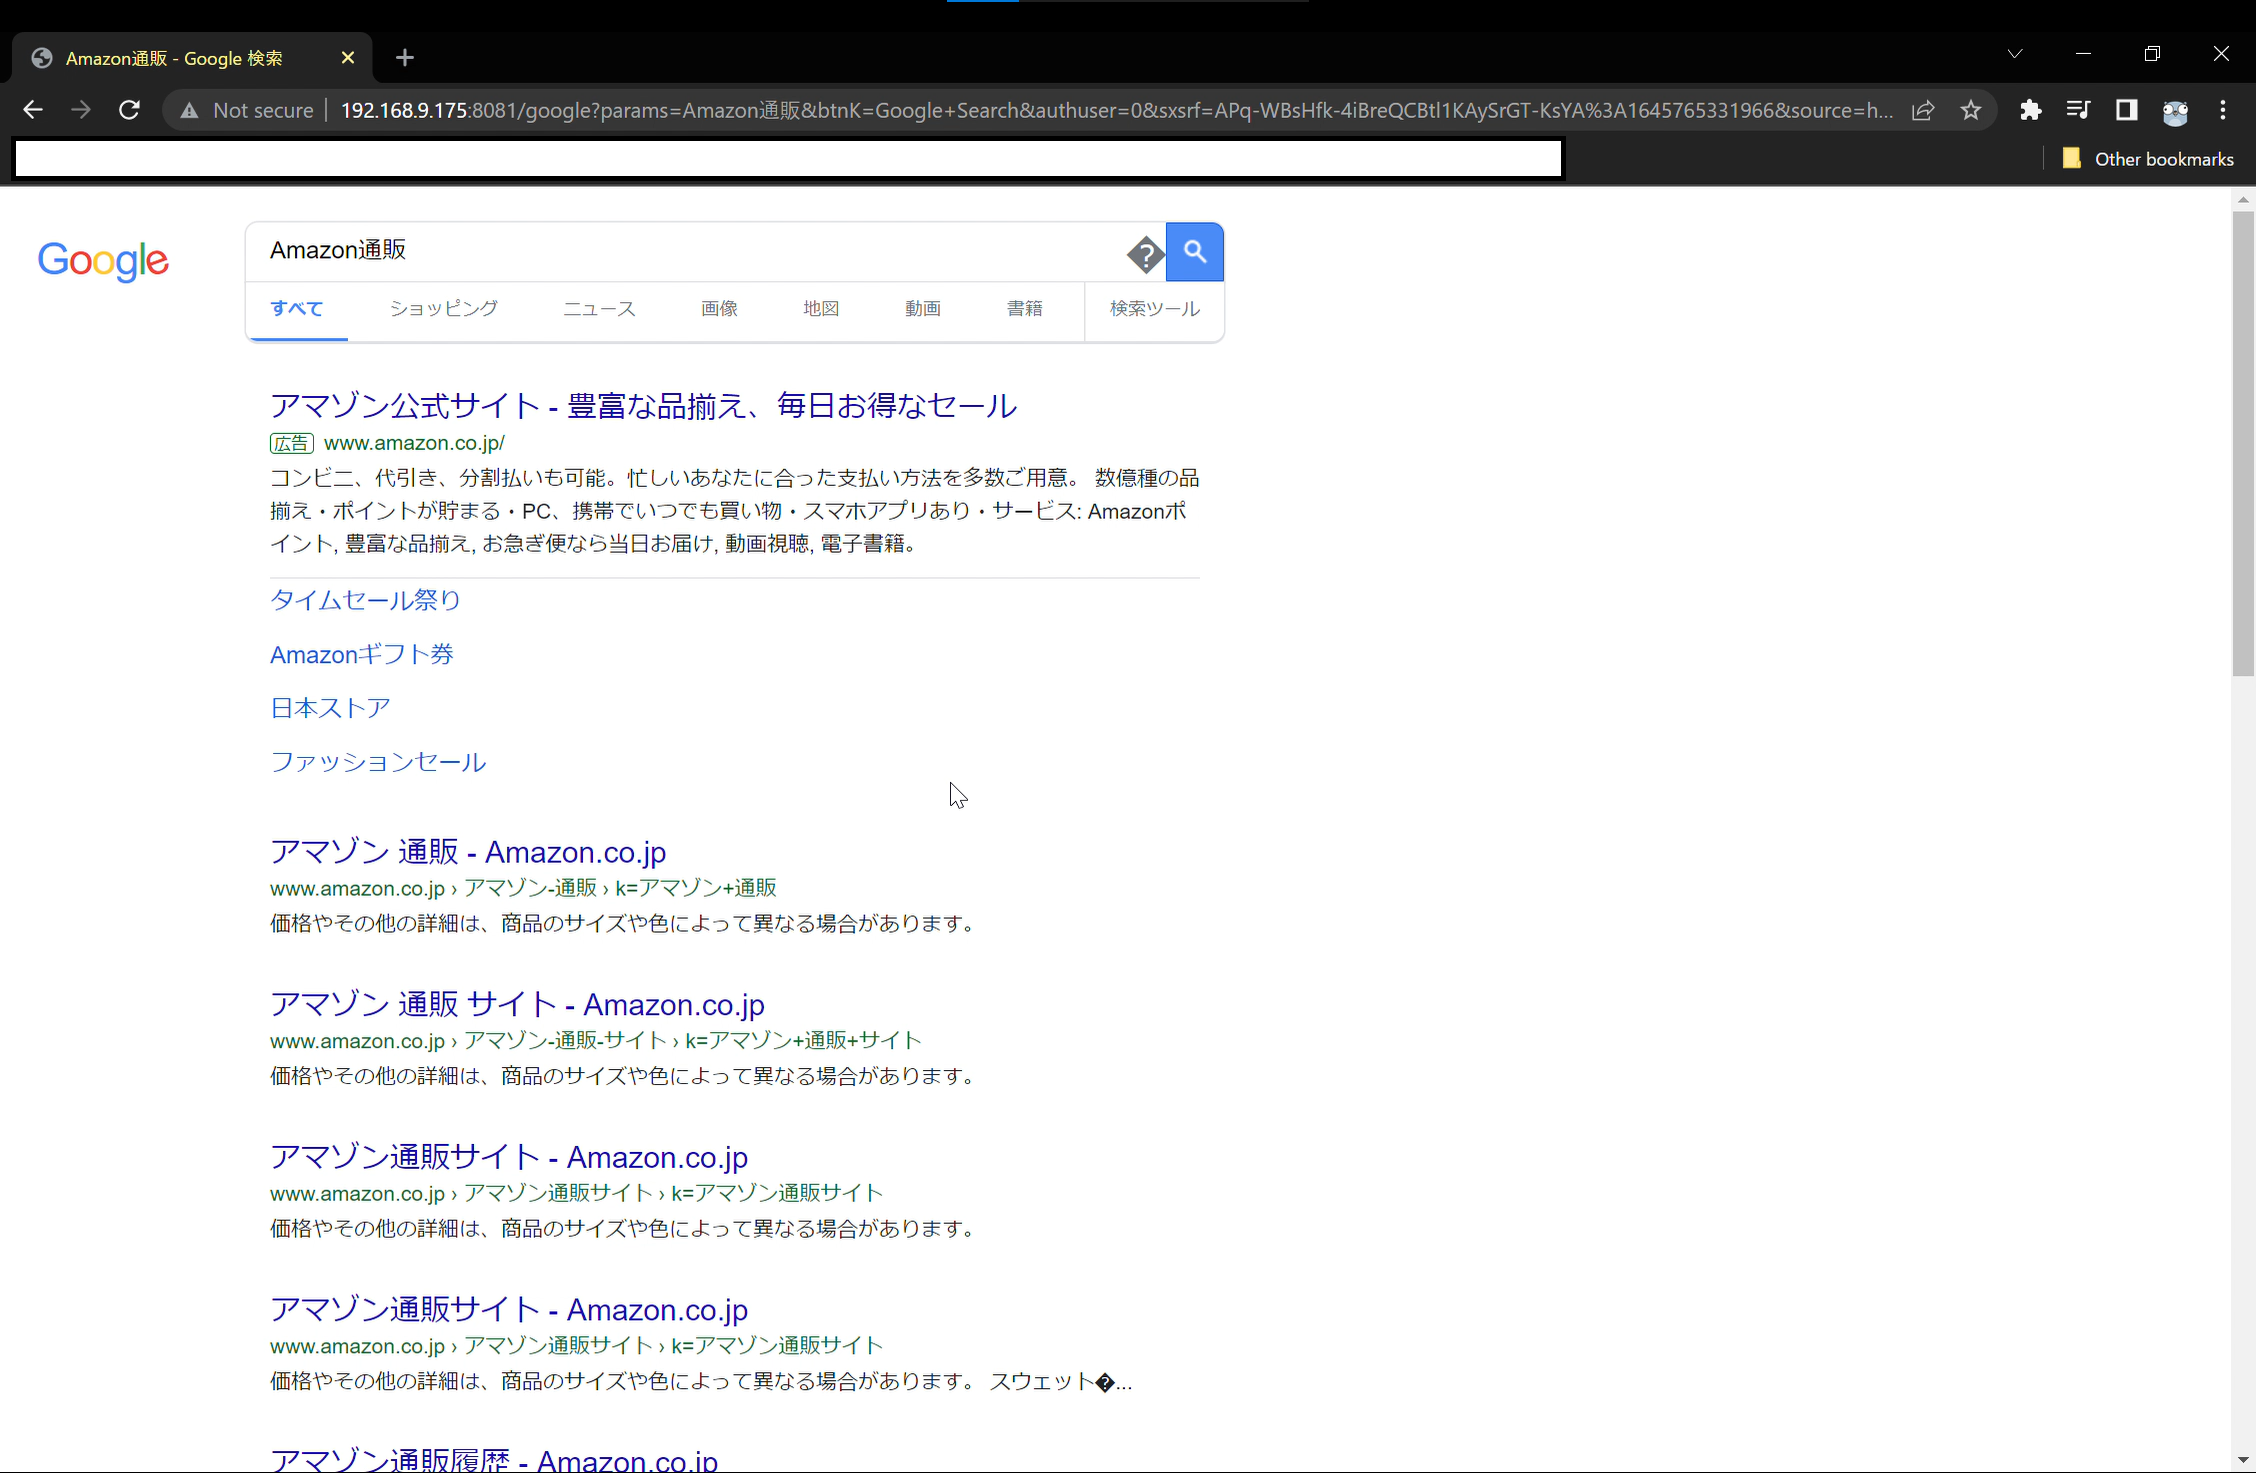
\includegraphics[height=7cm]{img/amazon/amazon-00.png}
                        \caption{「Amazon通販」と検索した際の画面}
                        \label{amazon-00}
                    \end{figure}
                    \\
                     取得した検索結果から複製されたAmazonの通販サイトに遷移した.\
                    続いて,ログインを行う為に画面右上にあるログインボタンを押して個人アカウントへの侵入に試みた.\
                    \begin{figure}[pth]
                        \centering
                        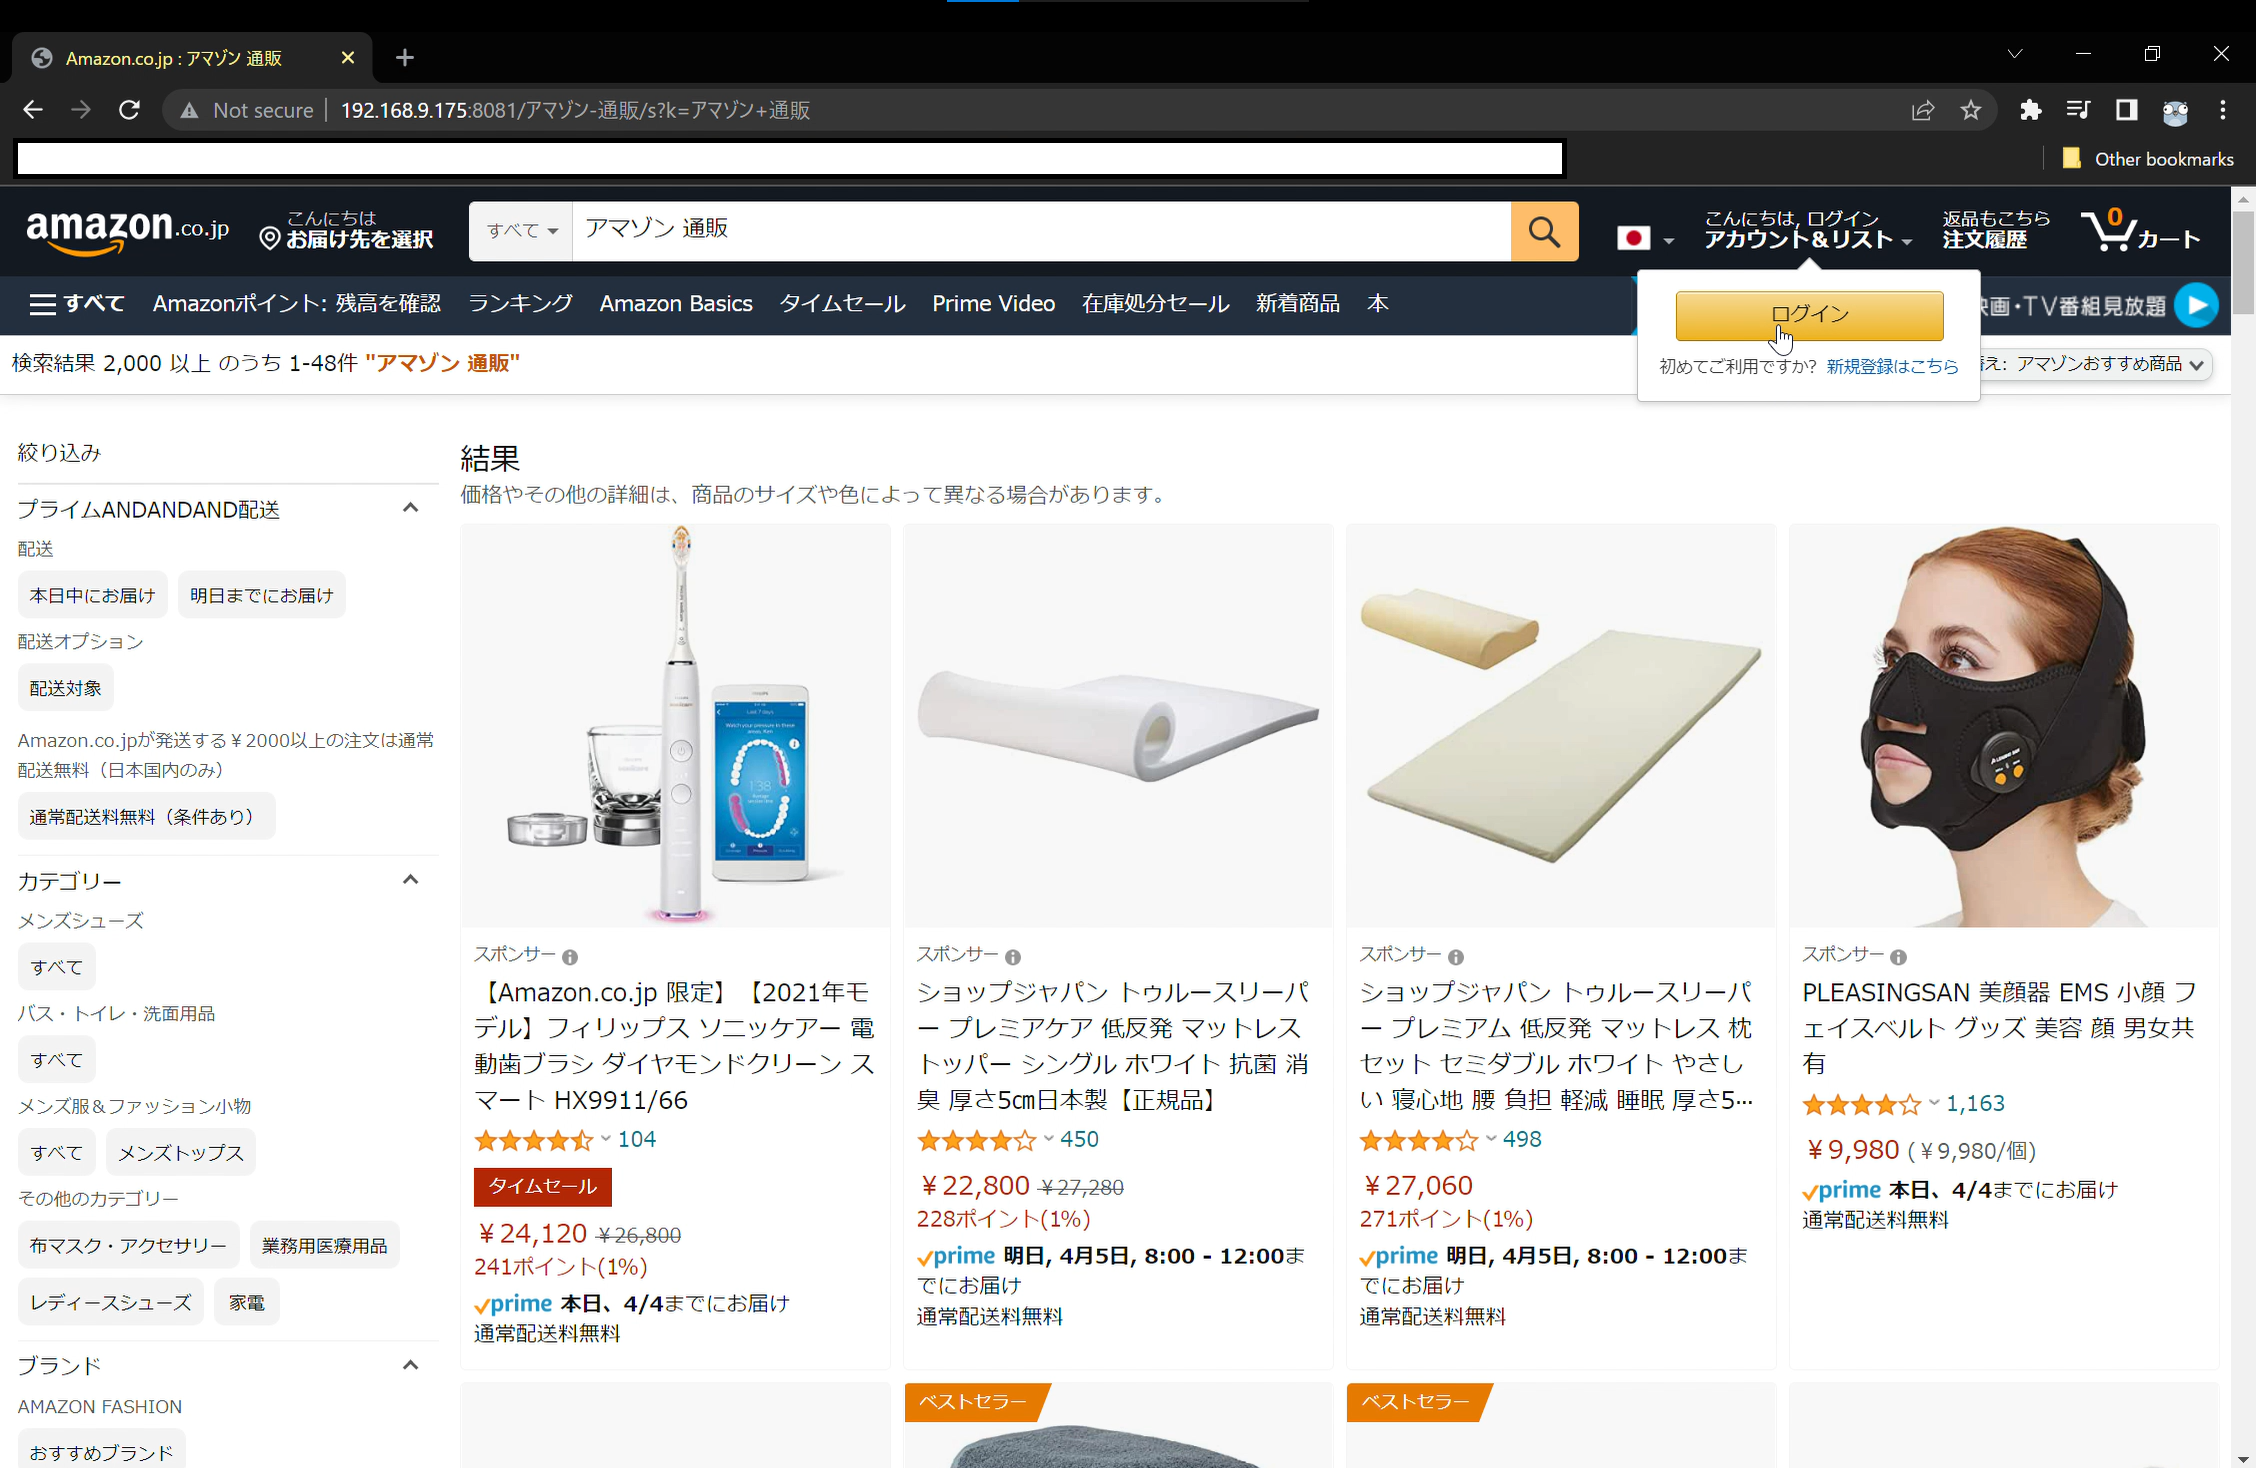
\includegraphics[height=7cm]{img/amazon/amazon-01.png}
                        \caption{検索結果の画面からAmazonの複製サイトへ遷移した際の画面}
                        \label{amazon-01}
                    \end{figure}
                    \clearpage
                     ログインボタンを押すと,ログイン画面に遷移した.\
                    この画面は予め攻撃者側で作成したもので.入力フォームとその入力データの送信を悪性サーバ側で取得するようにしている.\
                    この入力フォームに,実際にアカウント情報を入力してログインボタンを押した(図\ref{amazon-02}).\
                    \begin{figure}[pth]
                        \centering
                        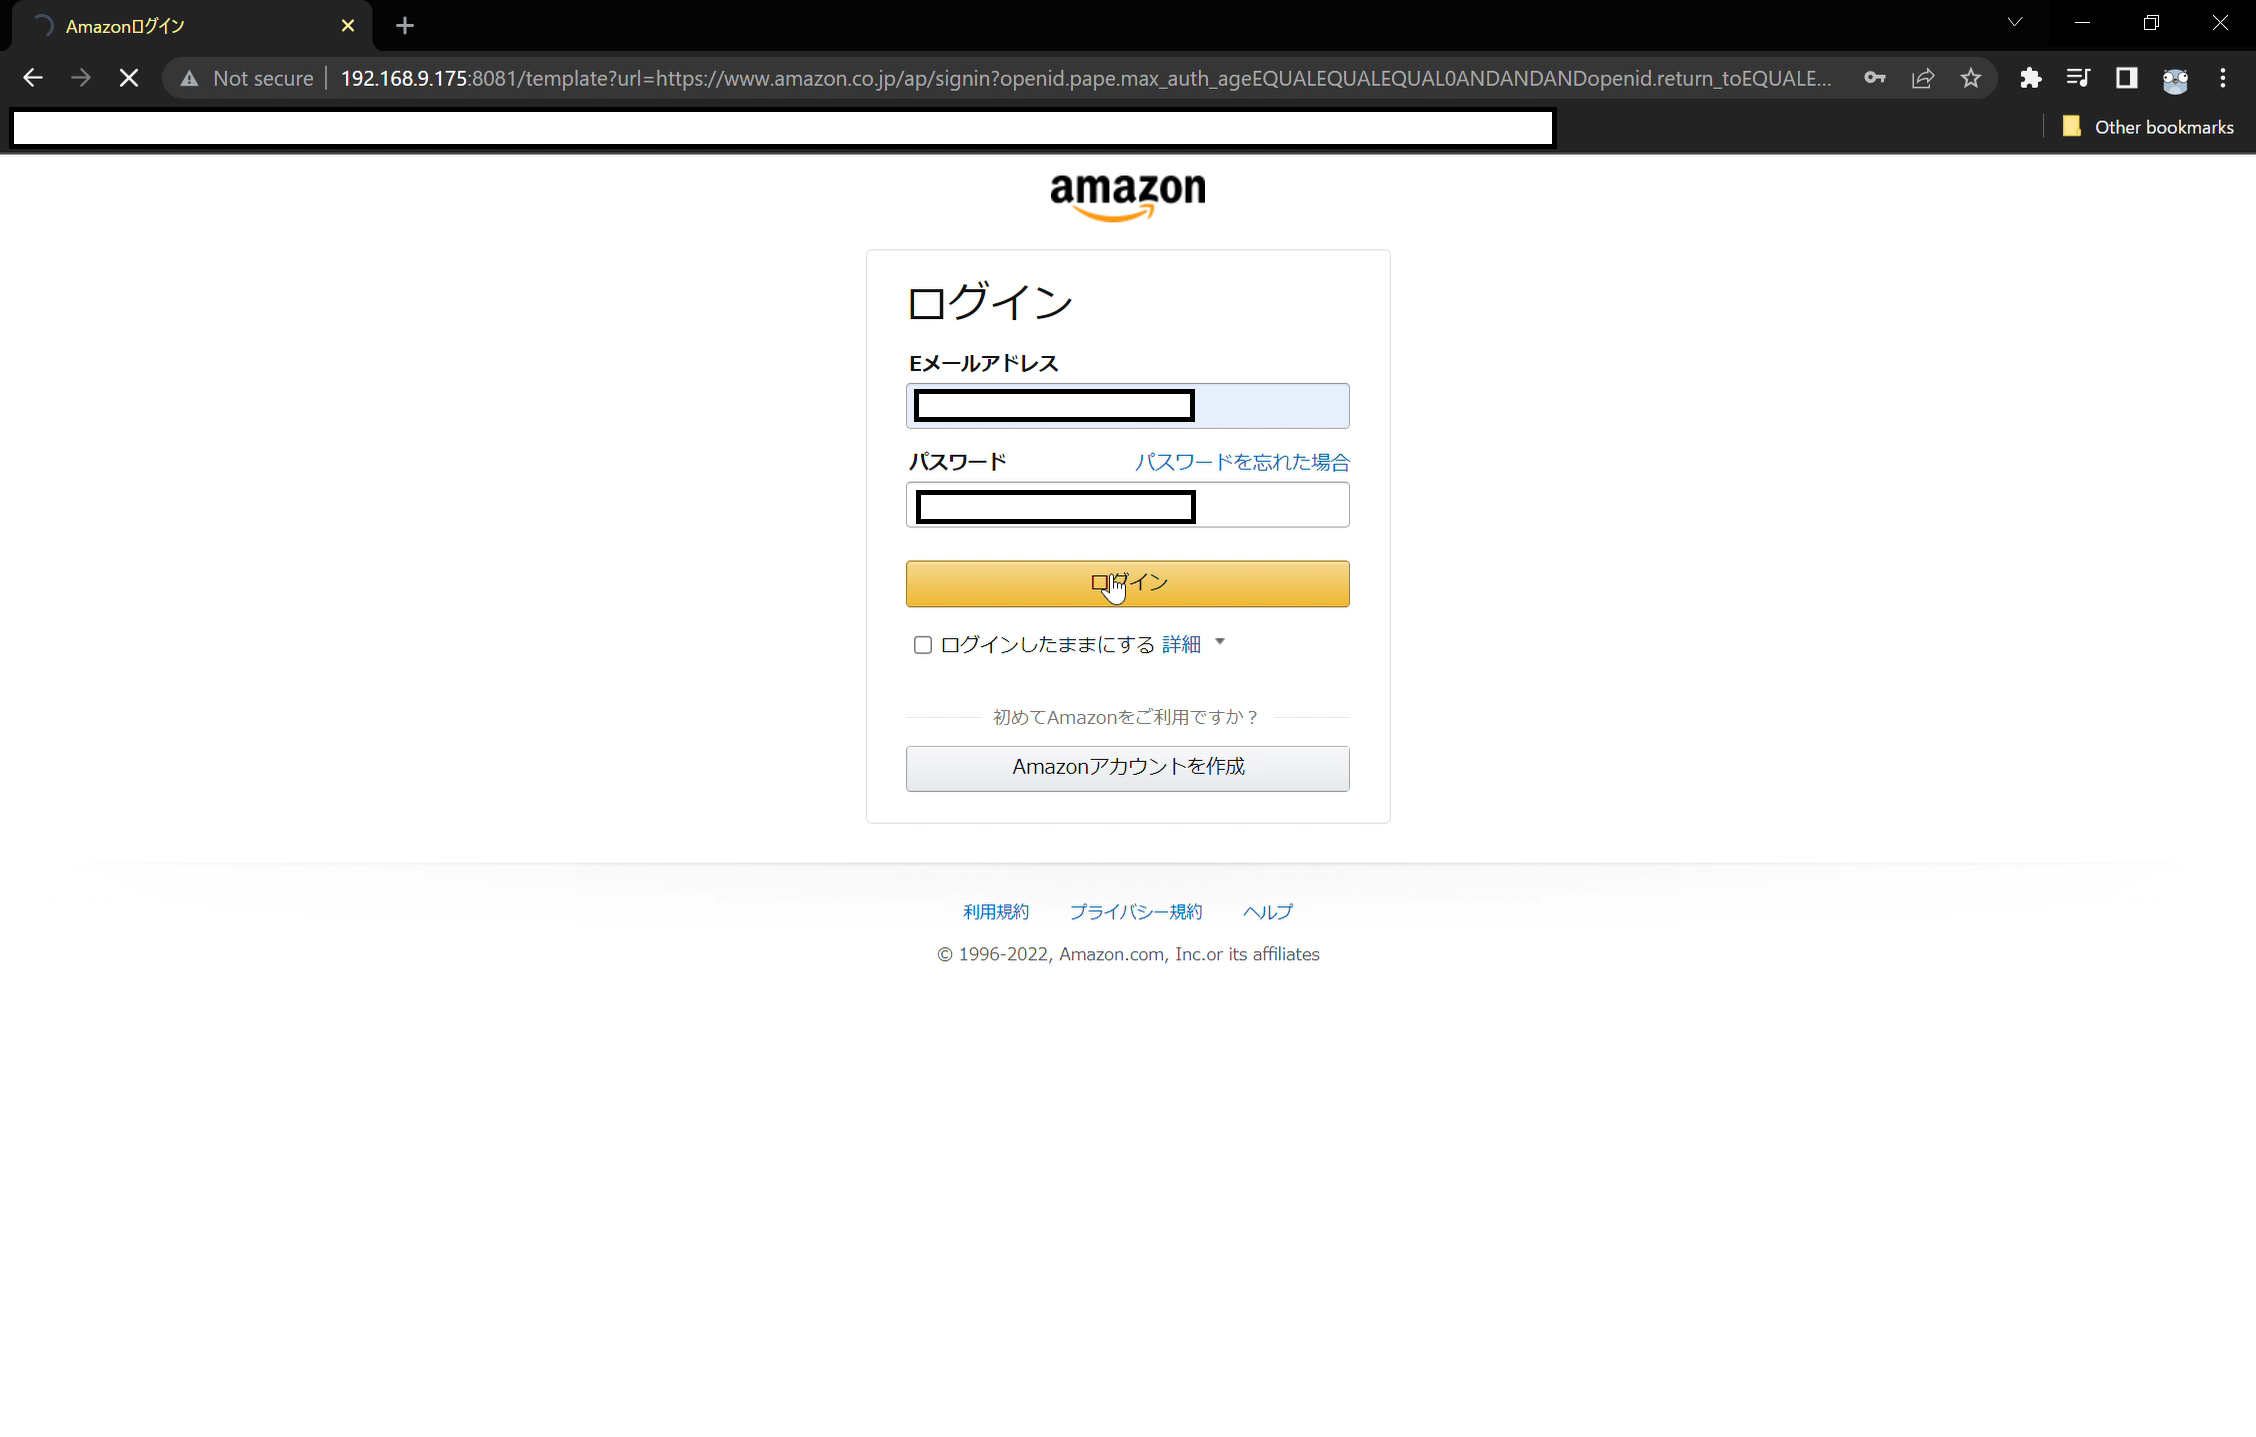
\includegraphics[height=7cm]{img/amazon/amazon-02.png}
                        \caption{ログイン画面へ入り,登録情報を入力した際の画面}
                        \label{amazon-02}
                    \end{figure}
                    \\
                     入力情報をサーバ側で取得して,図\ref{flow-6-7}の手順に従い入力情報の処理を行った.\
                    そして,入力情報の整合性の確認が完了し,実際に個人アカウントへの侵入に成功した.\
                    図\ref{amazon-03}の右上には,実際に個人アカウントの名前が明記されていることが分かる.\
                    ここまでの動作は図\ref{flow-6-7}の動作に準じて処理されたおり,楽天と同様に目立った画像切れや警告を出さずに,且つ正規サーバとの通信を攻撃者が中継する形で個人アカウントに侵入することができた.\
                    \begin{figure}[pth]
                        \centering
                        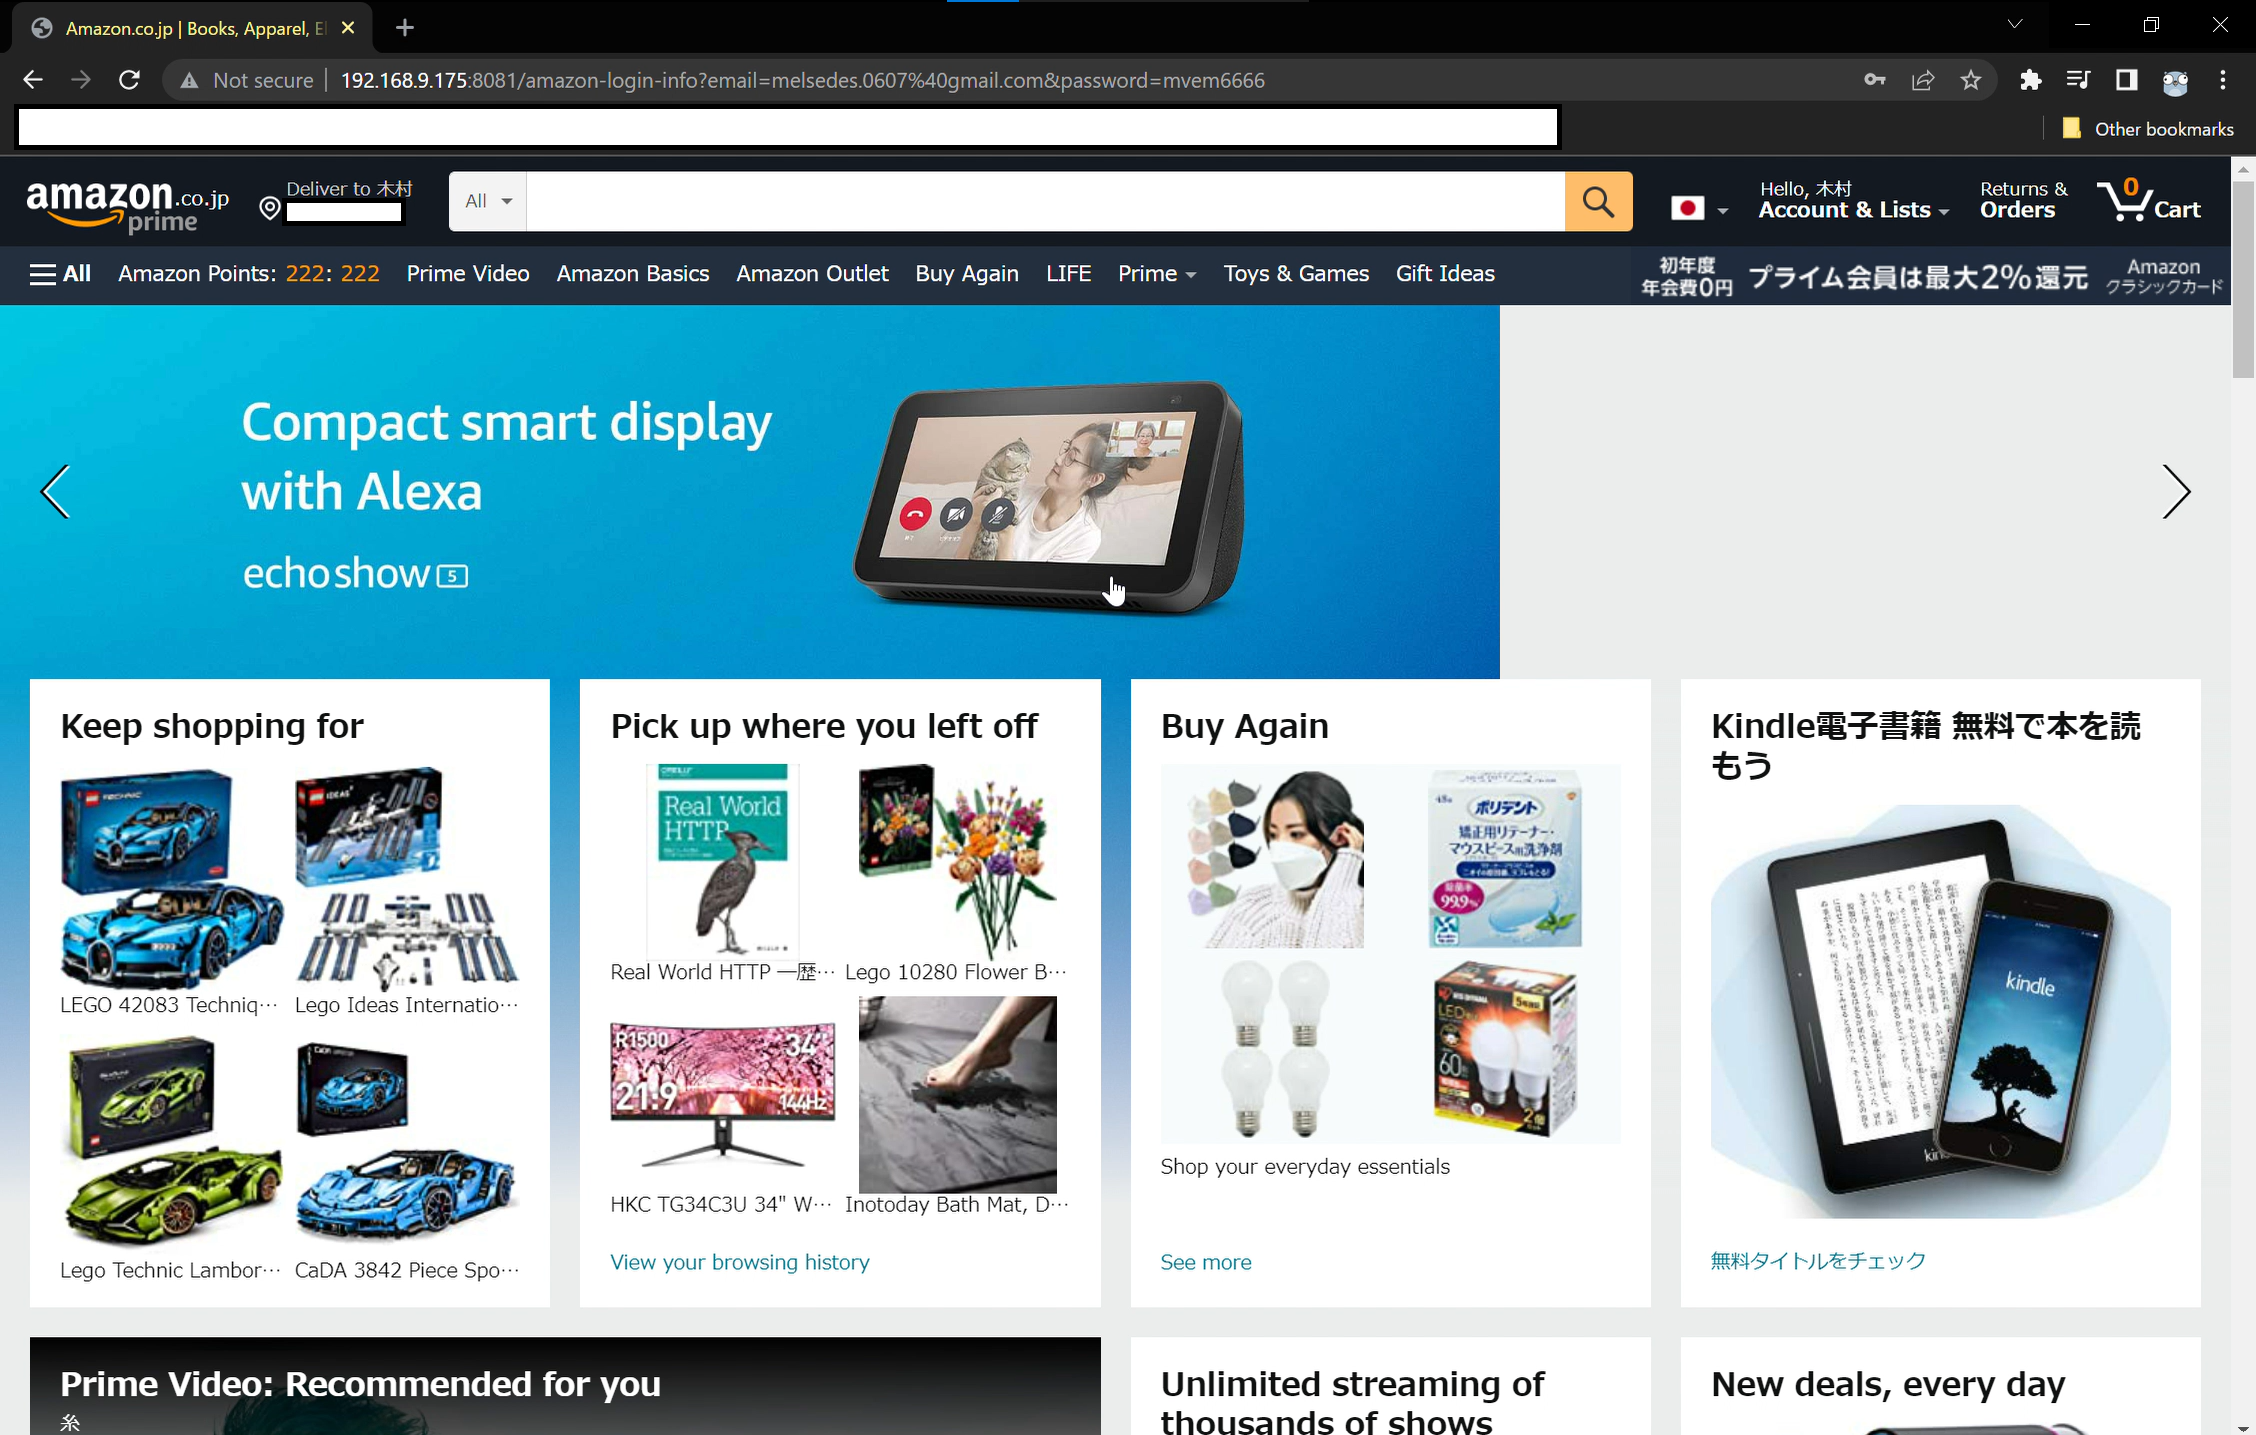
\includegraphics[width=7cm]{img/amazon/amazon-03.png}
                        \caption{ログイン情報の整合が取れ,実際に個人アカウントへログインした後の画面}
                        \label{amazon-03}
                    \end{figure}
                    \clearpage
                \subsubsection{問題点}
                    Amazonの場合,場合によればCAPTCHAに引っかかりログイン画面を突破できない場合があるという問題点が挙げられる.\
                    CAPTCHAとは,自動化されたボットによるWebサイトの操作を防止するもので,例えば,人間は認識可能でボットには認識不可能な歪みを含んだ文字列を提示し,その文字列を入力させる事で人間かボットかを認識するようなものが挙げられる(図\ref{captcha}).\
                    今回の実装では,CAPTCHAを回避或いはCAPTCHAの文字列を被害者に入力させて突破させる事はできなかった.\
                    \begin{figure}[pth]
                        \centering
                        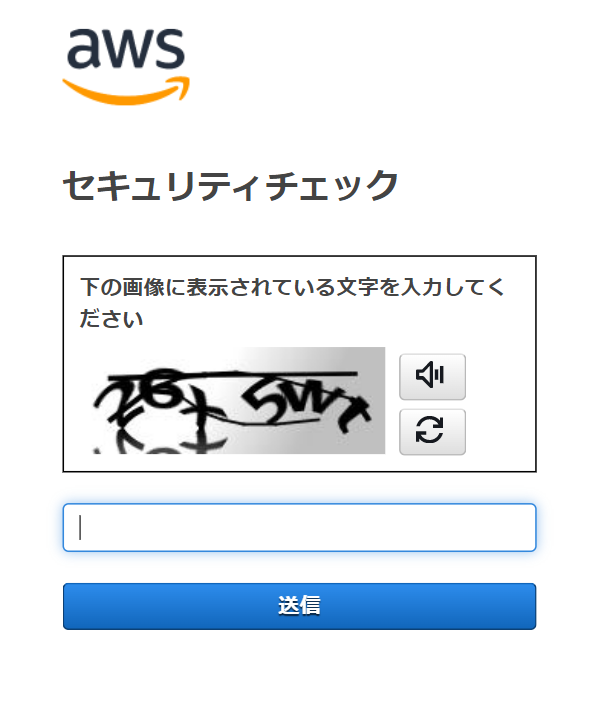
\includegraphics[height=7cm]{img/captcha.png}
                        \caption{CAPTCHAの例:AWSコンソールにログインする際に実際に出るCAPTCHAの一例}
                        \label{captcha}
                    \end{figure}
                    \clearpage
        \section{システムの評価}
            今回,「楽天」と「Amazon」の二つの通販サイトに絞ってシステムの構築を行ったが,両者ともブラウザ上での警告を出さずに個人情報の傍受・窃取が可能であることが分かった.\
            加えて,被害者のブラウザに対しても明確な警告の表示や画像切れが見れなかった為,通信の中継としての役割を十分に担う事ができていると評価できる.\\
             しかし,いくつかの問題点も残されている.\
            前節の検証結果でも述べたものを改めて列挙すると,次のようになる.\
            \begin{enumerate}
                \item (楽天の場合)登録情報の整合性の確認にやや時間を要する点.
                \item (Amazonの場合)CAPTCHAに引っかかり,ログインできない場合がある点.
            \end{enumerate}
             まず1についてであるが,これは6.1.2問題点にも記述したように,Chromedpを利用して個人情報の整合性の確認を行う際に非常に時間を要している点が主な原因と考えられる.\
            具体的な処理プロセスは,(1)Chromeインスタンスの作成,(2)ブラウザを開き楽天のログイン画面へ遷移,(3)指定のJS Pathを検索し個人情報を入力,(4)ログイン,(5)得られた結果をHTMLとして抽出,の計5行程となってるが.ログイン後の結果を完全に取得しようとした際,(4)と(5)の行程で約13秒程度待機する必要がある点が主なボトルネックとなっている.\
            今後の課題としては,Chromedpに依存していない部分の実行時間の削減に加え,今回の処理が別の言語で実行できる場合,Golangの場合との実行時間の比較を行い,ボトルネックの解消の可能性を探る必要がある.\\
             続いて,2についてであるが,CAPTCHAに引っかかる主な原因は,個人情報をプログラムで入力している点が原因である.\
            ブラウザ情報を維持したChromeインスタンスをCAPTCHAの回避を目的として再度別の処理で再利用する場合,Chromeインスタンスのリロードが必要となる.\
            しかし,Chromeインスタンスのリロードはブラウザ画面のリロードと同様の挙動を示すため,その際にCHATCHAとして表示された文字列も変わってしまう.\
            従って,被害者がCAPTCHAの文字列を入力したとしても,結果的に整合性が取れない.\
            現在,このCAPTCHAの問題を解決する具体的な実装はできていない為,今後も回避方法を考えていく必要がある.\
        \section{セキュリティ対策に関する考察}
            今回の結果から,Captive Portalを起点とする事で,通信の中継及び個人情報などの機密性・重要性の高い情報の傍受・窃取が可能になる事が分かった.\
            公衆無線LANの整備が進み,その利用場面に出会う回数が増えるに従い,インターネット利用に際する認証要求の経験は,至極当たり前のUXとして溶け込んでいく可能性が高い.\
            つまり,本研究の様なCaptive Portalによる認証から,認証後に別のページへ遷移するというUXも,日常的な経験からそのAPが偽物であるという想定もされなくなる可能性があり,依然として公衆無線LANを起点としたセキュリティの脅威は無くならないと考えられる.\
            本節では,本研究の様なCaptive Portalを起点としたセキュリティの脅威に対する対策方法を列挙・考察する.\
            具体的な対策方法は次の様なものが列挙できる.\
            \\
            \begin{enumerate}
                \item[対策 1] APの提供元が正規のものか確認する.
                \item[対策 2] 認証後のリダイレクトページからは,極力インターネットを利用しない.
                \item[対策 3] 認証後のリダイレクトページからインターネットを利用する際は,その通信先(主にドメイン)を確認し,正規のURLでない,
            \end{enumerate}
            \subsection{対策 1について}
                 対策1に関しては,本研究のCaptive Portalを起点としたセキュリティ脅威に関係無く,公衆無線LANを利用する際に利用者が注意を払うべき点である.\
            \subsection{対策 2について}
                 対策2に関しては,対策1ができなかった場合の対策である.\
                つまり,その提供元を確認せずに誤って悪意あるAPに接続してしまった場合の対策となっている.\
                Captive Portalによる認証終了後,そのAPの提供元が何らかのWebサイトに遷移するように設定している場合がある.\
                この時,利用しているAPが悪意あるものであった場合,攻撃者にとって複製された偽のWebサイトに利用者を遷移させる事は容易い.\
                公衆無線LANを用いる動機として,SNSの利用と共にWebサイトの利用はその筆頭であり,その窓口として検索エンジンの利用は必須である.\
                本研究のように,もし提示された検索エンジンが偽物だった場合,そこを起点として通信の中継が可能になってしまう.\
                このような事態を回避する方法は,認証後に遷移したWebサイトから離れ,そのサーバとセッションを切断する事である.\
                特に,本研究で行った検証の様な場面の場合,偽の検索エンジンに遷移させられたとしても,そのページを離れる事で,少なくとも直接的に通信の中継をさせる事は回避できる.\
            \subsection{対策 3について}
                 対策3に関しては,対策1及び対策2ができなかった場合の対策である.\
                透過型プロキシサーバーを利用する場合を除き,正規サーバではなく攻撃者サーバが通信を仲介する形の場合,利用者が閲覧しているサイトのドメインは,正規サーバではなく攻撃者サーバのものとなっている.\
                利用者は,この通信先のドメインを確認する事で,現在閲覧しているサイトが正規のものか否かを判別する事ができる.\
                今回の検証を例に挙げる場合,図\ref{compare-amazon-domain}し示した,正規と偽物のAmazonサイトのドメインを比較すると分かりやすい.\
                このように,公衆無線LAN経由で現在閲覧しているサイトが正規のものか否かを判別する事は,ドメインを確認する事で利用者側で判別することができる.\
                しかし,「前提知識・用語」の節でも挙げたように,フィッシング報告の状況からドメインの確認を利用者側に委ねる事は現実的に厳しいと考えられる為,対策2まででセキュリティ脅威を排除しておくことが望ましいと考えられる,\
                \begin{figure}[pth]
                    \centering
                    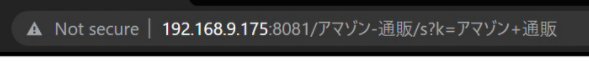
\includegraphics[width=10cm]{img/measure-domain-00.png}
                    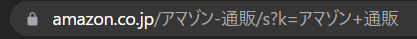
\includegraphics[width=10cm]{img/measure-domain-01.png}
                    \caption{Amazonサイトのドメイン比較(上:偽物 下:本物)}
                    \label{compare-amazon-domain}
                \end{figure}
        \section{参考文献}
            \begin{thebibliography}{9}
                \bibitem{SoumuWiFi} 総務省,2020年に向け全国約3万箇所のWi-Fi整備を目指して,\url{https://www.soumu.go.jp/main_content/000548781.pdf}
                \bibitem{IPA} IPA,公衆無線LAN利用に係る脅威と対策 ~公衆無線LANを安全に利用するために~,\url{https://www.ipa.go.jp/files/000051453.pdf}
                \bibitem{AboutMITM} オライリージャパン,渋川きよし 著,Real World HTTP ―歴史とコードに学ぶインターネットとウェブ技術 第2班,14.4 中間者攻撃(MITM攻撃)
                \bibitem{AboutHTML} Ohmsha,井上直哉・村山公保・竹下隆史・荒井透・苅田幸雄 共著,マスタリングTCP/IP 入門編 第6班,8.5.4 HTML(HyperText Markup Language)
                \bibitem{GoogleChromeHelp} Google Chrome ヘルプ,安全でないサイトについての警告表示を設定する,\url{https://support.google.com/chrome/answer/99020?hl=ja&co=GENIE.Platform%3DDesktop}
                \bibitem{Fishing} フィッシング対策協議会,2022年02 フィッシング報告状況,\url{https://www.antiphishing.jp/report/monthly/202202.html}
            \end{thebibliography}
        
        \section{付録}
            \subsection{実装コード}
                実装コードのGitHubリポジトリ \url{https://github.com/ES3-Kobe-U/go-malproxy}
            \subsection{Chromedp}
                ChromedpのGitHUbリポジトリ \url{https://github.com/chromedp/chromedp}
\end{document}